\chapter{Методы реконструкции случайных коэффициентов стохастического дифференциального уравнения Ито}
\label{ch:Methods}

\section{Обзор литературы}
\label{sec:ch1/Literature}

Одной из главных задач современной метеорологии, океанографии и климатологии является понимание того, как взаимодействуют тепловые потоки, температура поверхности моря и приземное атмосферное давление. Анализируя изменчивость и физические характеристики тепловых потоков и их взаимосвязь с другими метеорологическими переменными, можно получить ценную информацию о климатической системе Земли. Эти знания имеют решающее значение для улучшения средне- и долгосрочного прогнозирования погоды. Это позволяет более точно предсказывать появление экстремальных событий, таких как тропические ураганы, цунами и т.д. Кроме того, это помогает понять антропогенное воздействие на окружающую среду и различные другие факторы, влияющие на климат нашей планеты.

Потоки тепла между океаном и атмосферой тесно связаны с величиной SST (Sea Surface Temperature) -- температурой поверхности океана, оказывающей влияние на региональный климат. Известно, что большая часть изменчивости SST определяется именно рассматриваемыми поверхностными тепловыми потоками~\cite{schneider2015atmospheric,hausmann2017mechanisms,li2019decadal,blein2022parametrizing}. Существует целый ряд вопросов и проблем при количественной оценке тепловых потоков в процессе взаимодействия океана и атмосферы. Важно понять, где локально и как изменяются те области, в которых происходит максимальное взаимодействие, где количественно больше идет отток в атмосферу или наоборот поступление тепла и влаги из атмосферы, а где тепло больше перераспределяется внутри океана. Как это меняется по сезонам? Есть ли межгодовые тренды и колебания? Все эти вопросы окончательных ответов не имеют и более того, даже их постановка не является корректной в отсутствии адекватных моделей для описания процессов взаимодействия.

Известно, что на поверхности раздела двух сред -- океана и атмосферы -- турбулентные потоки тепла имеют высокую волатильность на различных пространственно-временных масштабах (\cite{small2019air,tian2017air}).  Турбулентные потоки вносят значительный вклад в изменчивость общего стока в межгодовом масштабе времени \cite{bentamy2017review}.
В работах \cite{ashin2019observed, schmeisser2019role} была изучена взаимосвязь между динамикой океана и изменчивостью температуры в смешанном слое в разных регионах. Теплообмен между океаном и атмосферой тесно связан с температурой поверхности океана, который оказывает значительное влияние на региональный климат. Также известно, что большая часть изменчивости температуры поверхности определяется именно поверхностными тепловыми потоками \cite{patrizio2021quantifying}. 
Поведение циклонов и их взаимосвязь с SST и тепловыми потоками, а также связь между приземным атмосферным давлением и тепловыми потоками были рассмотрены в работе \cite{tilinina2018association}. 

Взаимосвязь между аномалиями в явных и скрытых тепловых потоках и значениями SST над районами Северной Атлантики и Северной части Тихого океана была исследована в работе  \cite{cayan1992latent}. Роль условий преобразования энергии изо дня в день в течение жизненного цикла Североатлантического колебания, которое оказывает существенное влияние на погоду и климат в различных временных масштабах рассматривалась в работе  \cite{kim2024phase}. Была исследована реакция поверхностного слоя океана на неглубокую конвекцию в атмосфере \cite{brilouet2024numerical}. Изменчивость в Североатлантическом европейском регионе рассматривалась с использованием модели только для атмосферы, основанной на смещениях SST \cite{keeley2012impact}. 

Вероятностные результаты в данной области касаются аппроксимации распределения данных потоков тепла двухпараметрическим распределением Фишера--Триппета с оценкой его параметров по данным базы реанализа NCEP--NCAR за период 1948-2008 гг.~\cite{gulev2012probability}. В статье~\cite{FAO} изучено статистическое поведение экстремальных характеристик потоков (максимум, минимум) по области за весь период наблюдений в точках одноградусной сетки при различных осреднениях от суточных до годовых, а также средних значений по распределению и медиан. Кроме того, проведена аппроксимация вероятностных распределений для каждого из типов потоков тепла по отдельности и исследованы их совместные распределения.

Наиболее часто для анализа используются данные различных баз реанализа, содержащие аппроксимации реальных наблюдений~\cite{cronin2019air,leyba2019trends} на основе некоторых характерных значений для контактных сред. В данной статье в качестве данных для стохастической аппроксимации выступают элементы открытой базы реанализа ERA5\footnote{https://www.ecmwf.int/en/forecasts/datasets/reanalysis-datasets/era5}, формируемой Европейским центром среднесрочных прогнозов погоды.

Для изучения динамики процессов с учетом случайных факторов традиционным инструментом является аппарат случайных процессов. В физике плазмы~\cite{Espinos2018,Sexty2019} и финансовой математике~\cite{Bouchaud1998} хорошо известно стохастическое дифференциальное уравнение (СДУ) Ито (см. формулу~\eqref{eq:Ito} далее). Однако в области климатологии модели на его основе используются лишь в небольшом количестве работ для описания процессов, протекающих в океане. В работе ~\cite{van2021characterisation} были проведены исследования изменчивости явных и скрытых потоков, их экстремальных и средних значений в внутри- и межгодовом масштабе на основе данных из базы данных ERA5. Совместное поведение явных и скрытых потоков, их тренды и ковариационные функции в различных пространственно-временных масштабах изучались в работе ~\cite{toppaladoddi2021stochastic}. 

Первые исследования среднегодового хода явных потоков тепла по данным реанализа базы ERA5~\cite{hersbach2020era5} за $2010$--$2020$~гг. с использованием СДУ Ито были проведены авторами данного исследования в статье~\cite{2021_SOME_FEATURES}. В ней были изучены статистические закономерности внутригодовой и межгодовой изменчивости с различными масштабами усреднения: дневным, месячным, годовым. Также рассматривалось поведение экстремальных и средних потоков. В частности, показано существование положительного тренда максимума скрытого потока с течением времени. 

При построении количественных оценок тепловых потоков в системе океан-атмосфера большой интерес представляют вопросы о зонах со значительным взаимодействием и соответствующих местных характеристиках, а также о сезонных эффектах и межгодовых тенденциях и колебаниях.
\begin{itemize}
	\item Как меняются области, где происходит наиболее значимое взаимодействие, и каковы локальные характеристики этих областей?
	\item Где происходит количественный отток в атмосферу или, наоборот, поступление тепла и влаги из атмосферы, и где тепло в большей степени перераспределяется внутри океана?
	\item Как эти эффекты меняются в зависимости от времени года?
	\item Существуют ли межгодовые тенденции и колебания? Как изменения в тепловых потоках, температуре поверхности моря и атмосферном давлении проявляются количественно в различных масштабах пространства и времени?
	\item Существуют ли какие-либо изолированные океанские структуры, такие как квазициклонические или антициклонические вихри, где эти процессы взаимодействия можно в какой-то степени считать стационарными?
\end{itemize}
На эти вопросы нет однозначных ответов, и, более того, даже их формулировка может быть некорректной без адекватных математических моделей для описания процессов взаимодействия.
Такие вопросы рассматриваются и решаются в численных гидродинамических моделях, которые моделируют взаимодействие океана и атмосферы~\cite{gulev2012probability}.
Однако эти модели в значительной степени зависят от трудно поддающихся оценке внешних и внутренних факторов: коэффициентов вязкости, уровней турбулентности и скоростей обмена. Эти факторы либо неизвестны, либо их трудно определить на основе наблюдений. Кроме того, существует зависимость от начальных и граничных условий, которые также сложно определить. Некоторые компромиссы основаны на моделях, которые включают в себя ассимиляцию данных~\cite{FAO}. Однако, даже в случаях усвоения данных расчеты для долгосрочных периодов требуют установки дополнительных параметров.

В данной работе в качестве модели динамики изменчивости теплового потока в системе воздух-море используется хорошо известное стохастическое дифференциальное уравнение (СДУ) Ито \cite{Pascucci2022}. Задача оценки (вообще говоря) случайных коэффициентов СДУ, учитывая наблюдения за процессом, предполагает некоторые существенные допущения относительно математических свойств коэффициентов \cite{Yoshida1992, GenonCatalot1993, GenonCatalot1994, Wei2016}. В упомянутых работах авторы предполагают, что коэффициенты являются функциями неизвестного параметра $\theta$; некоторые из них даже предполагают определенный тип зависимости от этого параметра. В работе \cite{FlorensZmirou1993} рассмотрен непараметрический случай, и оценка коэффициента диффузии, наряду с доказательством его сходимости и непротиворечивости, получена в предположении существования трех непрерывных ограниченных производных этого коэффициента, а также неслучайности и существования ограниченных производных коэффициента дрейфа. Также можно использовать основанный на ядре метод регрессии \cite{Lamouroux2009}.

Применение модели Ито для оценки эволюции приращения теплового потока было ранее рассмотрено в работе \cite{2021_SOME_FEATURES}. Модель СДУ Ито обобщает хорошо известные статистические модели динамики климата, в частности, модели Будыко \cite{Budyko1974} и Хассельмана \cite{Hasselmann1976}. Эта модель также представлена в работах \cite{van2021characterisation, toppaladoddi2021stochastic}, где авторы использовали ее для описания поведения тепловых потоков между льдом и океаном в Арктическом регионе. Статистические особенности модели в двумерном случае были подробно рассмотрены в \cite{Pascucci2022}. Оценка неизвестного параметра модели в многомерном случае уравнения Ланжевена, являющегося вариантом уравнения Ито, была предложена в работе \cite{Voutilainen2022}.

Параметр дрейфа в уравнении Ито соответствует средним изменениям в поведении системы с течением времени, зависящим как от конкретного момента времени, так и от величины потока. Выявление областей, где этот коэффициент является значительным, может быть полезно для определения зон струйных течений, фронтов и синоптических вихрей, где происходят значительные динамические процессы. Области с малым коэффициентом дрейфа и большим стохастическим (диффузионным) коэффициентом соответствуют областям сильной турбулентности, включая энергетически активные области в Северной Атлантике. Поэтому задача оценки параметров стохастической модели поведения приращения тепловых потоков важна для решения задач с точки зрения математического моделирования.

Моделирование приращений потоков (в отличие от традиционно используемого для изучения значений самих потоков) адекватно описывает динамику потоков в среднесрочной и долгосрочной перспективе и, по-видимому, хорошо согласуется с реальными данными. Эта модель имеет ряд преимуществ перед известными численными или стохастическими моделями. Она довольно проста, поскольку форма модели определяется двумя коэффициентами, даже в многомерном случае (вектор дрейфа и матрица диффузии). Таким образом, можно количественно оценить поведение изучаемых характеристик, т.е. проанализировать и спрогнозировать их. Кроме того, эта схема является довольно общей, поскольку она включает как динамические модели со случайным воздействием (т.е. внешним воздействием), так и модели, основанные на тенденциях в периодических и случайных компонентах. Предлагаемая модель использует хорошо развитый аппарат теории стохастических дифференциальных уравнений и параболических уравнений Фоккера-Планка–Колмогорова, поэтому она удобна, например, для количественных и качественных оценок динамики потоков, их пространственно–временной изменчивости и вероятностей возникновения редких, но опасных событий, тропические ураганы.


\section{Математическая модель}
\label{sec:Model}

Рассмотрим динамико-стохастическую модель вида
\begin{equation}
	\label{eq:Ito}
	dX = a(t,X)\,dt + b(t, X)\,dW(t), 
\end{equation}
называемую стохастическим дифференциальным уравнением Ито.

Модель~\eqref{eq:Ito} используется для описания случайных процессов диффузионного типа, в которых изменчивость самого процесса за малый промежуток времени мала по сравнению с изменчивостью его среднего значения и дисперсии~\cite{jin2020controls,van2021characterisation}. В таком случае за указанный малый промежуток времени эта изменчивость может рассматриваться как сумма квази-детерминированного процесса, определяемого сносом $a(t, X)$ (здесь термин <<квази>> учитывает наличие зависимости непосредственно от случайного процесса $X$), и чисто случайного процесса $b(t, X)$, не зависящего от первого слагаемого и определяемого диффузионной составляющей.

В формуле~\eqref{eq:Ito} $X = (X_1(t), X_2(t))$ -- двумерный случайный процесс, значения которого в фиксированный момент времени $t$ имеют смысл вектора значений двух рассматриваемых физических величин в рассматриваемой географической точке, $a(t,X)$ и $b(t,X)$ –- случайные коэффициенты сноса и диффузии, зависящие от времени и значения потока, $dW(t)$ -- винеровский процесс, не зависящий от процесса $X$. Первая компонента векторного коэффициента переноса $a(t, X)=(a_1(t,X), a_2(t,X))$ соответствует первой, а вторая -- второй переменной из рассматриваемой пары. Для определения коэффициента $b$ рассмотрим оператор диффузии $B(t, x)$ с собственными значениями $\lambda_i(t, x), i=1,2$ и соответствующими собственными векторами $e_i(t, x), i=1,2$. Положим
\begin{equation}
	\label{b_vector}
	b_i(t,x) = \sqrt{\lambda_i(t, x)}e_i(t, x), \quad i=1,2,
\end{equation}
и объединим эти два вектора в матрицу. Коэффициентом $b(t, X)$ будем называть матрицу $2\times2$ со случайными значениями:
\begin{equation}
	\label{eq:b_coeff}
	b(t,X) =  \begin{bmatrix}  
		b_{11}(t, X) & b_{12}(t, X) \\
		b_{21}(t, X) & b_{22}(t, X)
	\end{bmatrix}
\end{equation}
Здесь $b_{ii}(t, X)$ -- соответственно диффузионные компоненты первой и второй величин из рассматриваемой пары (например, явный и скрытый потоки тепла, давление и температура поверхности моря и т.д.), а $b_{12}(t,X)$ и $b_{21}(t,X)$ описывают взаимодействие величин, представляя собой в некотором смысле аналог ковариации. Однако, вообще говоря, $b_{12} \neq b_{21}$.

Решение СДУ \eqref{eq:Ito} представляет собой диффузионный процесс с матричным  коэффициентом диффузии $b^2(t, X)$ и векторным коэффициентом сдвига (или дрейфа) $a(t,X)$. При этом случайные коэффициенты $a(t,X)$ и $b^2(t,X)$ представляют собой условное математическое ожидание и дисперсию приращений потока соответственно:
\begin{equation}
	\label{eq:a_coeff_E}
	a(t,X)= \frac{\E(X(t+dt)-X(t)|X(t)=x)}{dt},
\end{equation}
\begin{equation}
	\label{eq:b_coeff_D}
	b^2(t,X)= \frac{\D(X(t+dt)-X(t)|X(t)=x)}{dt},
\end{equation}
где E и D - математическое ожидание и дисперсия случайной величины соответственно.

Для существования решения уравнения~\eqref{eq:Ito} необходимо выполнение некоторых условий~\cite{Skorohod} на рассматриваемые борелевские функции $a(t, x)$ и $b_i(t, x), i=1,2$. В приложении~\ref{app:Existance} проведена проверка справедливости этих условий для изучаемых данных реанализа пары явного и скрытого потоков тепла с целью обоснования корректности применения математической модели. Можно продемонстрировать, что для этих данных выполняются условия существования решения СДУ (см. книгу~\cite{Skorohod}, стр. 469). %Почему убрали про однозначное определение свойств временного ряда? Мне кажется, здесь было бы уместно

При отсутствии априорной информации о физической структуре процесса $X(t)$ проблема статистического восстановления функций $a(t)$ и $b(t)$ становится одной из важнейших. Из-за их случайной природы эта задача допускает, по крайней мере, два принципиально различных подхода к ее постановке. Первый из них заключается в получении оценок (которые сами по себе были бы случайными) функций $a(t)$ и $b(t)$, то есть в построении их точечных приближений. Второй подход представляет собой статистическую реконструкцию случайных коэффициентов $a(t)$ и $b(t)$ в терминах их распределений. То есть, зная некоторые свойства этих коэффициентов, можно найти оценки некоторых числовых параметров этих моделей. Оба подхода можно интерпретировать как физически реалистичные и осуществимые.

\section{Непараметрический метод оценивания}
\label{sec:Nonparametic}
Ключевым предположением при изучении рассматриваемых данных реанализа является предположение, что все их статистические характеристики зависят только от самих значений и не зависят от точки локализации. Иными словами, это допущение того, что значения потока, взятые в разных точках пространства, можно считать принадлежащими одной и той же генеральной совокупности с присущей ей некоторыми статистическими характеристиками. Это предположение вполне обосновано, так как традиционные расчетные формулы для потоков~\cite{cronin2019air,leyba2019trends} используют только сами значения контактных сред, но не их локацию. Поэтому при достаточно больших размерах рассматриваемой области для каждого интервала значений потоков тепла, от минимального до максимального значения потоков в фиксированную дату, найдется достаточно много пространственных точек, и соответственно значений потоков, чтобы оценка вероятности перехода значений потока из одного состояния в другое за небольшой отрезок времени была состоятельна \todo{ссылка}.


\subsection{Дискретизация данных}
\label{sec:Discretization}
Для применения непараметрического метода оценивания случайных коэффициентов дрифта и диффузии СДУ Ито~\eqref{eq:Ito} требуется предварительно перейти от формально бесконечного множества возможных значений процесса к конечному множеству. Далее представлено краткое описание этого процесса для одномерного случая, в многомерном случае алгоритм выполняется для каждой из компонент независимо.

Рассмотрим два соседних момента времени $t_1$ и $t_2$. Для того, чтобы оценить коэффициенты $a(t,x)$ и $b(t,x)$, потребуется определить значения переходных вероятностей процесса с использованием только множества значений в эти соседние моменты времени, поскольку не предполагается однородность процесса. Но в таком случае, учитывая вещественность значений, при фиксации значения $x$ в момент времени $t_1$ ему будет соответствовать, скорее всего, лишь одна географическая точка сетки, в которой достигается это значение. В таком случае соответствующее значение $y$ в момент времени $t_2$ будет единственным отвечающим состоянием с вероятностью перехода, равной $1$, что нельзя считать адекватной оценкой для описания переходов процесса. Поэтому необходимо разбить весь диапазон значений процесса в выборке на непересекающиеся интервалы и заменить все значения, попадающие в каждый из интервалов, на какое-то общее значение. Наиболее естественным способом для этого является использование квантилей для построения интервалов с одинаковыми вероятностями попадания в них, с учетом описанного выше предположения локальной однородности данных.

Итак, независимо для каждого элемента рассматриваемой пары $(X_1(t), X_2(t))$ за некоторый период времени рассматриваются все известные значения. Выбирая $N$ точек (например, $N=1000$) $\left\lbrace p_1, \ldots, p_{N} \right\rbrace $, разделяющих  отрезок $[0, 1]$ на части одинаковой длины, для каждого $p_i$ находится квантиль соответствующего порядка $q_i$, $i=1, \ldots, N$. Затем каждое значение одномерного процесса ($X_1$ или $X_2$), попавшее в интервал $[q_i, q_{i+1}]$, заменяется величиной $(q_i + q_{i+1})/2$. В некотором смысле это похоже на процесс приближения абсолютно-непрерывной случайной величины с помощью дискретной.

Таким образом множество всех значений ряда за рассматриваемый достаточно большой промежуток времени (например, 10 лет ежедневных измерений) сводится к конечному (небольшому) множеству. Как было отмечено в разделе \ref{sec:ch1/Literature}, для получения данных реанализа используются только сами значения контактных сред, но не их местоположение. Поэтому при достаточно больших размерах географической области для каждого интервала значений рассматриваемой физической величины от минимального до максимального значения в фиксированный момент времени найдется достаточно много пространственных точек и, соответственно, значений величины, чтобы оценка вероятности перехода процесса из одного состояния в другое за небольшой отрезок времени была состоятельна. 

\subsection{Формулы}
Для каждого фиксированного момента времени точечные оценки функций $a(t,x)$ и $b(t,x)$ могут быть построены только на основе значения рассматриваемого двумерного процесса $X = (X_1(t), X_2(t))$. А именно, для построения оценок в момент времени $t+1$ требуется на основе выборки по всей рассматриваемой географической области оценить вероятности перехода процесса $X(t)$ из каждого элемента множества его значений в момент $t$ в каждый элемент множества значений в момент $t+1$. Будем обозначать значения процесса с помощью строчных букв.

В случае дискретных значений процесса рассмотрим условную вероятность $\P(y|x) = \P(X(t+dt)=y|X(t)=x)$, а в абсолютно-непрерывном случае -- плотность $p(y|x)dx = p(y<X(t)|x < X(t) = x)$. Тогда коэффициенты $a(t, x)$ и $b(t, x)$ для некоторых фиксированных значений двух элементов случайного процесса
$x = (x_1, x_2)$ %и $y = (y_1, y_2)$
определяются \cite{Skorohod} формулами
\begin{gather}
	\label{eq:a_formula_0}
	a_i(t,x_i) = \lim_{\varDelta t \to 0} \frac{1}{\varDelta t} \int\limits_{t}^{t+\varDelta t} (y_i-x_i)p(y_i|x_i)\,dy, \quad i = 1,2;\\
	\label{eq:b_formula_0}
	b_{i, j}^2(t, {x}) = \lim_{\varDelta t \to 0} \frac{1}{\varDelta t} \int\limits_{t}^{t+\varDelta t} (y_i-x_j)(y_i-x_j)^T p(y|x)\,dy, \quad i,j = 1,2.
\end{gather}

Таким образом, для оценки коэффициентов $a(t,x)$ и $b(t,x)$ необходимо оценить переходные вероятности, фигурирующие в правой части формул~\eqref{eq:a_formula_0}--\eqref{eq:b_formula_0} под знаком интеграла. На практике рассматривается процесс с дискретным временем, измерения которого проводятся через фиксированный промежуток времени $\varDelta t$, поэтому предел в правой части равенств~\eqref{eq:a_formula_0}--\eqref{eq:b_formula_0} исчезает, кроме того, с учетом конечности выборки измерений процесса, интегралы заменяются на конечные суммы. 

Далее необходимо провести дискретизацию процесса по алгоритму, описанному в разделе~\ref{sec:Discretization}. Обозначим полученное множество возможных значений как $X_1, X_2, \dots, X_{N}$, где $X_i = (q_i + q_{i+1})/2$. Далее для каждого $t \in [0, T-1]$ оценим вероятности перехода процесса из одного состояния в другое:
\begin{equation}
	\label{eq:p_formula}
	p_{ij} = \frac{\#\{X(t) = X_i, X(t+1) = X_j\}}{\#\{X(t) = X_i\},}
\end{equation}
где символ $\#$ обозначает количество элементов в соответствующем множестве, $j = 1,\ldots,N$, $i \in \{1, \dots, N\}: \#\{X(t) = X_i\} > 0$. Очевидно, что при этом для $i$, соответствующих непустому набору в момент времени $t$, $\sum\limits_{j=1}^{N} p_{ij} = 1$. Эту процедуру можно выполнить как рассматривая один элемент пары в оба момента времени, так и разные элементы пары, получая с учетом порядка $4$ набора вероятностей. Обозначим эти наборы, соответственно, $P_{1-1}, P_{1-2}, P_{2-1}, P_{2-2}$. 

Оценки для коэффициента переноса $a(t,x)$ в момент времени $t \in [0, T-1]$ в точках, соответствующих значению одномерного компонента процесса ($X_1$ или $X_2$) $x_i \in \{X_1, \dots, X_{N}\}$, строятся следующим образом:  
\begin{equation}
	\label{eq:a_formula}
	a_{x_i} = \sum\limits_{j=1}^{N} (x_i - y)\cdot p_{ij}, \quad x_i, y \in \{X_1, \dots, X_{N}\}, 
\end{equation}
где $p_{ij}$ берется по одному из наборов $P_{1-1}$ для первого элемента пары или $P_{2-2}$ для второго. Таким образом, в момент времени $t$ в каждой географической точке определён вектор точечных оценок $a = (a_1, a_2)$.

Оценки квадрата коэффициента диффузии строятся аналогичным образом, но с некоторыми различиями. Во-первых, в каждой географической точке в момент времени $t$ предварительно оценивается матрица размера $2 \times 2$:
\begin{equation}
	\label{eq:b_coeff_est}
	b_t(x_{1,i}, x_{2, i}) =  \begin{bmatrix}  
		b_{11} & b_{12}\\
		b_{21} & b_{22}
	\end{bmatrix},
\end{equation}
где $x_{1, i}$ -- значение первой компоненты в рассматриваемой точке в момент времени $t$, а $x_{2, i}$ -- значение второй компоненты в этой же точке. Обозначим через $X_{first}$ и $X_{second}$ множества значений рассматриваемой пары в момент времени $t$, а через $Y_{first}$ и $Y_{second}$ -- множества значений пары в момент времени $t+1$. Тогда:
\begin{gather}
	\label{eq:b_formula}
	b_{k,l, i} = \sum_{j=1}^{N} (x_{k, i} - y_l)^2 \cdot p_{ij}, 
\end{gather}
где $k=1,2$ и $l=1,2$ - два индекса, соответствующие первому и второму элементу пары в момент времени $t$ и $t+1$, соответственно, $x_1 \in X_{first}, x_2 \in X_{second}, y_1 \in Y_{first}, y_2 \in Y_{second}$. Нетрудно заметить, что при получении оценок для компонент матрицы суммируются квадраты разностей. Искомые оценки для коэффициента диффузии получаются извлечением матричного корня из полученной матрицы $b_t(x_{1,i}, x_{2, i})$.

При этом при реализации данного подхода периодически, хотя и довольно редко, появлялись ситуации, когда оцененная матрица в точке не обладала свойством положительной определенности. В таких случаях в найденной матрице-корне на побочной диагонали возникали комплексные значения. Было принято решение в таких случаях для этих чисел отбрасывать мнимую часть и сохранять только действительную, отрицательную часть. Поэтому, вопреки интуитивным ожиданиям, минимум шкалы значений оценок для коэффициента диффузии в некоторых случаях мог быть отрицательным.

Данная процедура описана в виде алгоритма (блок-схемы) в разделе~\ref{sec:ComponentsAlgo}. Там же приводится оценка его вычислительной сложности и обсуждаются детали программной реализации разработанного пакета стохастического анализа потоков между океаном и атмосферой. 

\section{Полупараметрический метод оценивания}
\label{sec:Semiparametric}
Как было отмечено выше, непараметрический метод имеет строгие теоретические обоснования, однако он требует выполнения некоторого набора условий для коэффициентов, которые часто не могут быть проверены на реальных геофизических данных. Альтернативным рассматриваемым подходом является полупараметрический статистический метод, основанный на реконструкции распределений неизвестных случайных коэффициентов дрейфа и диффузии, который подразумевает, что процесс оценки выполняется с использованием разделения сдвиг-масштабных конечных смесей нормальных законов. Стоит отметить, что в случае неслучайных коэффициентов рассматриваемого СДУ Ито~\eqref{eq:Ito} при принятии дополнительных предположений об измеримости в отношении естественной фильтрации и нормальности распределения начального значения процесса, решением оказывается некоторый гауссовский процесс с заданным средним значением и ковариационной функцией. Строгая теоретическая постановка задачи сходимости для полупараметрического метода сложна. В данной работе полупараметрический подход, свободный от каких-либо дополнительных допущений, сравнивается с непараметрическим, чтобы продемонстрировать близость результатов и, как следствие, корректность его применения. Одно из важных потенциальных применений полупараметрического метода связано с задачей прогнозирования. В его рамках возникают теоретически обоснованные аппроксимации распределений для решений СДУ Ито. Эти распределения, или, скорее, параметры и компоненты связности, полученные в результате их оценки, могут быть использованы в рамках физически-информированного машинного обучения. Некоторые примеры эффективного улучшения прогнозов нейронной сети с использованием этого метода были продемонстрированы ранее в \cite{Kuzmin2022} для нескольких тепловых потоков в Лабрадорском море и Гольфстриме. Стоит отметить, что для получения точечных оценок с помощью первого подхода в данном случае может потребоваться решение нескольких СДУ.


Известно~\cite{Skorohod}, что для СДУ Ито~\ref{eq:Ito} с неслучайными коэффициентами при дополнительных предположениях об измеримости процесса в отношении естественной фильтрации и нормальности распределения начального значения решение имеет вид некоторого гауссовского процесса с заданным средним и ковариационной функцией. В этой ситуации приращения процесса также являются гауссовскими случайными величинами. Однако, если каждый параметр является случайным, естественным образом возникают распределения вида $\E \Phi (\frac{x-A}{B})$, то есть дисперсионно-сдвиговые смеси нормальных законов. Для данного метода более уместно говорить о восстановлении коэффициентов стохастического дифференциального уравнения, а не об их оценке. Предлагаемый полупараметрический подход позволяет реконструировать совместные одномерные распределения коэффициентов дрейфа и диффузии. Для этого выбирается часть исходного временного ряда (окно), и наблюдения в этом окне рассматриваются как однородная выборка. Теоретическое распределение этих наблюдений представляет собой нормальную смесь по шкале сдвига. Для математической корректности задачи непрерывные нормальные смеси аппроксимируются конечными нормальными смесями, которые можно идентифицировать~\cite{Teicher1961}. Следует отметить, что, в общем случае, задавая достаточно большое количество компонентов дискретной смеси, можно сделать аппроксимацию достаточно точной.

Формально, пусть $n \ge 1$, $t_0=0<t_1< ... <t_n$ - моменты времени, в которые известны значения процесса $X(t)$. Для простоты предположим, что $t_i - t_{i-1} = 1 \forall i\ge 1$. Как упоминалось выше, распределение приращений $X(t_i)-X(t_{i-1})$ процесса $X(t)$ может быть аппроксимировано непрерывными нормальными смесями:
$$
\label{eq:approx_diskr}
\P(X(t_i) - X(t_{i-1})<x) \approx \E \Phi\left(\frac{x-A_i}{B_i}\right),
$$
где $\Phi(x)$ - функция распределения стандартного нормального закона, а $A_i \in R$ и $B_i > 0$ - случайные величины. Аппроксимация конечными нормальными смесями выглядит следующим образом:
$$
\P(X(t_i) - X(t_{i-1})<x) \approx \sum\limits_{k=1}^K p_k \Phi\left(\frac{x-a_k}{b_k}\right),
$$
где $K \in N$, $p_k \ge 0, k=1,..., K$, $\sum\limits_{k=1}^K p_k = 1$. Параметры $p_k$, $a_k$ и $b_k$ в формуле~\eqref{eq:approx_diskr} могут отличаться для моментов времени $t_i$ и $t_{i+1}$.

Для статистической оценки параметров $p_k$, $a_k$ и $b_k$ в формуле~\eqref{eq:approx_diskr} можно использовать метод скользящего разделения смесей. На основе выборки из окна выделяется конечная смесь, которая приблизительно соответствует теоретической смеси, то есть статистически определяются масштаб и параметры среднего компонент, а также их веса. Эти параметры определяют дискретную аппроксимацию совместного распределения коэффициентов.

Алгоритм максимизации математического ожидания (EM-алгоритм)~\cite{McLachlan2007} -- это хорошо известный итерационный метод получения оценок максимального правдоподобия, который может быть использован для параметров $p_k$, $a_k$ и $b_k$~\eqref{eq:approx_diskr}. Далее приведены явные формулы для параметров на итерационных этапах для рассматриваемого случая конечных нормальных смесей. 

Пусть $\phi(.)$ -- стандартная нормальная функция плотности вероятности. Переменные 
$$
g_{kj}^{(m)}= \frac{\frac{p_k^{(m)}}{\sigma_k^{(m)}} \phi\left(\frac{x_j - a_k^{(m)}}{\sigma_k^{(m)}} \right)}{\sum\limits_{r=1}^K \frac{p_r^{(m)}}{\sigma_r^{(m)}} \phi\left(\frac{x_j - a_r^{(m)}}{\sigma_r^{(m)}} \right)}
$$
являются апостериорными вероятностями того, что распределение случайной величины соответствует $i$-му компоненту смеси. Тогда параметры на $(m+1)$-й итерации определяются следующим образом ($i=1,...,K$; $n$ - размер выборки (окна)):
$$
p_k^{(m+1)} = \frac{1}{n} \sum\limits_{j=1}^n g_{kj}^{(m)},
$$
$$
a_k^{(m+1)} = \frac{1}{\sum\limits_{j=1}^n g_{kj}^{(m)}} \sum\limits_{j=1}^n g_{kj}^{(m)} x_j,
$$
$$
\sigma_k^{(m+1)} = \sqrt{\frac{1}{\sum\limits_{j=1}^n g_{kj}^{(m)}} \sum\limits_{j=1}^n g_{kj}^{(m)} (x_j - a_k^{(m+1)})^2}
$$
Хорошо известно, что лучшим среднеквадратичным предиктором квадратичной интегрируемой случайной величины является ее математическое ожидание. Поэтому в качестве предикторов или реконструкций коэффициентов используются взвешенные выборочные значения предельных распределений параметров сдвига и масштаба. Затем окно перемещается на один шаг вправо, и весь процесс повторяется. Таким образом, ширина окна, т.е. количество наблюдений в выборке окна, не должна быть слишком маленькой, чтобы гарантировать приемлемую точность оценок параметров смеси, и не должна быть слишком большой, чтобы предотвратить излишнее сглаживание. Последнее требование делает весьма проблематичной даже попытку поставить задачу изучения традиционных свойств реконструкций (или оценок) коэффициентов стохастического дифференциального уравнения, таких как асимптотическая несмещенность или согласованность. Действительно, эти свойства предполагают, что размер выборки, т.е. ширина окна в рассматриваемом случае, бесконечно растет, тогда как при увеличении ширины окна возрастает возможность не заметить существенных изменений в поведении стохастического процесса.

Для каждого набора точек, которые попадают в одну и ту же группу во время дискретизации~\ref{sec:Discretization} значений процесса $X(t)$, могут быть получены оценки среднего значения и дисперсии аппроксимирующей смеси, соответствующие желаемым оценкам коэффициентов $a(t,X)$ и $b(t,X)$. Для каждых двух матриц значений процесса $(X(t),X(t+1))$ на двух последовательных временных шагах получается соответствующая матрица $X_q(t)$ из процедуры дискретизации.


Как было упомянуто выше, элементы этой матрицы могут принимать только одно из $K$ различных значений из ранее построенного набора квантилей. Предполагается, что количество групп $K$ в данном методе намного меньше, чем в случае построения точечных оценок непараметрическим методом (см. раздел~\ref{sec:Nonparametic}), поскольку в этом случае для выбора групп с использованием дискретизации значения учитываются только в один момент времени $t$, в отличие от использования всех значений процесса матрица за весь период наблюдения $t \in \{0,...,T\}$. Каждому из квантилей $q \in \{q_1,..., q_K\}$ соответствует набор $\{(i_1, j_1), (i_2, j_2),..., (i_n, j_n)\}$ точек матрицы $X_q(t)$, соответствующих значению квантиля $q$. Это приводит к выборке $\{X[i_1,j_1 ], X[i_2,j_2 ],...,X[i_n,j_n]\}$ значений исходного процесса перед дискретизацией. После применения модификации алгоритма EM с предварительно заданным числом компонентов $N$ к построенной выборке, получаются соответствующие оценки максимального правдоподобия параметров каждого компонента (вектор среднего значения, дисперсии и веса $(a_i,\sigma_i^2, w_i), i=1,...,N)$.


Таким образом, в полупараметрическом методе оценки случайных коэффициентов СДУ Ито~\ref{eq:Ito} $a(t, X)$ и $b(t,X)$ в момент времени $t$ в точках с координатами $(i_1, j_1), (i_2,j_2),..., (i_n, j_n)$ задаются формулами:
$$
\hat{a}(t, i_m, j_m) = \sum\limits_{i=1}^N w_i a_i,
$$
$$
\hat{b^2}(t, i_m, j_m) = \sum\limits_{i=1}^N w_i (a_i^2 + \sigma_i^2),
$$
\subsection{Выделение компонент связности}
\label{sec:Components}
В силу природы непараметрического метода на каждом шаге (положении окна) выделяются компоненты аппроксимирующей смеси нормальных законов, которые затем усредняются с соответствующими весами, чтобы получить итоговые оценки случайных коэффициентов в целом. Однако исследование эволюции самих выделенных компонент представляет собой отдельную задачу, представляющую интерес с точки зрения природы физических процессов (примеры таких процессов можно найти в статье \cite{2020_statistical_estimation_Langevin}, где впервые описывается данный метод). В данном разделе очень кратко представлена суть метода выделения эволюции компонент, а в разделе~\ref{sec:ComponentsExamples} приведены иллюстрации его применения к реальным данным.

Итак, пусть $n\geq1$ и $t_0=0<t_1<\ldots<t_n$ -- моменты времени, в которые наблюдается процесс $X(t)$. Пусть $t_i-t_{i-1}=1$ для любого $i\geq1$. Из уравнения~\eqref{eq:Ito} видно, что распределение приращения $X(t_i)-X(t_{i-1})$ процесса $X(t)$ можно аппроксимировать распределением вида
\begin{equation}
	\label{eq:DiffApprox}
	\P\left(X(t_i)-X(t_{i-1})<x\right)\approx \E\Phi\left(\frac{x-A_i}{B_i}\right),
\end{equation}
где $\Phi(x)$ -- стандартная нормальная функция распределения,
$A_i\in\R$ и $B_i>0$ -- случайные величины. В свою очередь, для распределений случайных величин $A_i$ и $B_i$, по отношению к которым берется математическое ожидание в формуле~\eqref{eq:DiffApprox}, можно использовать дискретную аппроксимацию. Тогда вместо выражения~\eqref{eq:DiffApprox} для распределения приращения $X(t_i)-X(t_{i-1})$ можно применить приближение вида
\begin{equation}
	\label{eq:DiffDiscrApprox}
	\P\left(X(t_i)-X(t_{i-1})<x\right)\approx\sum_{k=1}^Kp_k\Phi\left(\frac{x-a_k}{b_k}\right),
\end{equation}
где $K\in\N$, $p_k\geq0$, $k=\overline{1,K}$, $\sum\limits_{k} p_k=1$. Очевидно, параметры $p_k$, $a_k$ и $b_k$, формирующие так называемые динамические и диффузионные компоненты~\cite{Korolev_book}, зависят также от $i$ и изменяются при переходе от $t_i$ к $t_{i+1}$.

Чтобы восстановить эволюцию распределения случайных функций $a(t)$ и $b(t)$ в целом, надо восстановить компоненты смеси~\eqref{eq:DiffDiscrApprox} как функции времени, то есть, решить задачу приближенного восстановления двумерного распределения $F_t(x,y)\equiv \P\left(a(t)<x,b(t)<y\right)$. С этой целью при каждом $i=\overline{1,n}$ ищется дискретная аппроксимация распределения $F_{t_i}(x,y)$, а затем осуществляется интерполяция этой функции для остальных $t$. Для интерполяции необходимо установить соответствие между множествами возможных значений $\{a_k,b_k: k=\overline{1,K}\}$ случайных коэффициентов $a(t_i)$ и $b(t_i)$ при разных $i$.

В процессе шагов СРС-метода выделяются компоненты смеси~\eqref{eq:DiffDiscrApprox}, которые эволюционируют при сдвигах скользящего окна. При этом достаточно сложно судить о том, какая из оценок параметров соответствует тому или иному значению на предыдущем шаге. Обычно подобная взаимосвязь определяется визуально и, очевидно, является достаточно субъективной. В статье \cite{2020_statistical_estimation_Langevin} был предложен подход к автоматизации решения данной задачи на основе комбинации жадного алгоритма и методов кластеризации $k$- или $c$-средних~\cite{steinhaus1956division,macqueen1967some,arthur2006k,dunn1973fuzzy}. На первом этапе определяется число кластеров для методов машинного обучения, которые используются непосредственно для выявления связанных компонент. Вопрос о качественном изменении рассматриваемых компонент в формулировке добавления шума к чистому сигналу рассматривался в работе \cite{gorshenin2020efficiency}.

Пусть $I^{(n)}$ -- набор индексов компонент для шага с номером $n$ СРС-метода, то есть $I^{(n)}=\{1,2,\ldots,k^{(n)}\}$, а $J^{(n+1)}=\{1,2,\ldots,k^{(n+1)}\}$ -- аналогичный набор для шага $(n+1)$. $I_0$ и $J_0$ представляют собой множество индексов из первого и второго наборов соответственно, для которых удалось найти ближайшую компоненту. Первоначально $I_0=\emptyset$ и $J_0=\emptyset$. Затем для каждого фиксированного $J\in J^{(n+1)}\setminus J_0$ находится наиболее близкий номер $I$ в смысле решения следующей оптимизационной задачи:
\begin{equation}
	\label{I}
	I=\argmin\limits_{i\in I^{(n)} \setminus I_0}\left(\left|a_i^{(n)}-a_J^{(n+1)}\right|^p+
	\left|\sigma_i^{(n)}-\sigma_J^{(n+1)}\right|^p \right)^{1/p}.
\end{equation}

В этом случае минимизируемое в правой части выражение представляет собой $\ell^p$-норму ($p=1,2,\ldots$) соответствующего вектора разностей координат в пространстве точек $(a,\sigma)$.

Полагая после этого $I_0=I_0\cup I$ и $J_0=J_0\cup J$, необходимо повторить процедуру заново. Возможны следующие случаи:
\begin{enumerate}
	\item $\left|I^{(n)}\right|=\left|J^{(n+1)}\right|$, то есть $k^{(n)}=k^{(n+1)}$. В этом случае оба набора будут исчерпаны одновременно;
	\item $\left|I^{(n)}\right|<\left|J^{(n+1)}\right|$, то есть $k^{(n)}<k^{(n+1)}$. В этом случае процедура останавливается, когда исчерпан набор $I^{(n)} \setminus I_0$. Оcтавшиеся в  $J^{(n+1)}\setminus J_0$ элементы формируют новые компоненты, которые появились только на $(n+1)$-м шаге.
\end{enumerate}

Случай $\left|I^{(n)}\right|>\left|J^{(n+1)}\right|$, то есть $k^{(n)}>k^{(n+1)}$, не рассматривается, поскольку основная цель данной процедуры -- определение числа компонент за весь период эволюции процесса.

Для точного определения числа компонент необходимо задавать некоторый допустимый порог близости $\varepsilon( a, {\boldsymbol \sigma})$:
\begin{equation}
	\label{Dist}
	\left(\left|a_I^{(n)}-a_J^{(n+1)}\right|^p+
	\left|\sigma_I^{(n)}-\sigma_J^{(n+1)}\right|^p +\left|p_I^{(n)}-p_J^{(n+1)}\right|^p\right)^{1/p} < \varepsilon({a}, {\boldsymbol \sigma}).
\end{equation}

Такая проверка нужна для того, чтобы корректно определять ситуацию, при которой компоненты с номерами $I$ и $J$ на $n$-м и $(n+1)$-м шагах считались одинаковыми, и не было необходимости создавать новую в рамках жадного алгоритма. Блок-схема метода определения числа компонент приведена далее в разделе ~\ref{sec:ComponentsAlgo}.


\section{Сравнение методов}
\label{sec:Compare}
Для проверки и сравнения точности описанных выше методов оценивания случайных коэффициентов СДУ Ито~\eqref{eq:Ito} генерируется реализация случайного процесса с заданными коэффициентами в виде линейной комбинации тригонометрических функций. Кроме того, проведено количественное сравнение предложенных методов по скрытым и явным тепловым потокам в Северной Атлантике с использованием данных реанализа из базы ERA5 за период $1979$--$2022$ гг. Показано, что результаты обоих методов довольно близки. В случаях некоторого расхождения в результатах предлагается геофизическая интерпретация.

\subsection{Модельные данные}
\label{sec:ModelData}
Результаты обоих рассмотренных статистических подходов можно сравнить на моделируемых случайных процессах, описываемых СДУ~\eqref{eq:Ito}, в терминах RMSE (среднеквадратичной ошибки):
$$
RMSE(\vec{x}, \vec{y}) = \sqrt{\sum\limits_{i=1}^n \frac{(x_i - y_i)^2}{n}}
$$

В качестве модельного распределения используется реализация процесса, соответствующего уравнению Ито~\eqref{eq:Ito}, с использованием заданных неслучайных функций $a(t,X)$ и $b(t,X)$ тригонометрического вида. Выбор тестовых функций такого типа основан на том факте, что реальные геофизические данные часто имеют годовой цикл и другие периодические компоненты. Поэтому при применении статистических методов важно быть уверенным, что эти методы хорошо воспроизводят наличие гармоник в данных. Итак, тестовые функции определяются следующим образом:
$$
a(t, X) = \sum\limits_{k=1}^M p_k cos(\omega t) \alpha X_{t-1},
$$
$$
b(t, X) = \sum\limits_{k=1}^M p_k cos(\omega t) \beta X_{t-1},
$$
где $w_k$ -- частоты $M$ рассматриваемых гармоник, а $p_k$ -- их веса, для которых выполняется ограничение $\sum\limits{k=1}^M p_k = 1$.

Для генерации данных, аналогичных формату географической карты, для проверки работоспособности алгоритмов берется несколько гармоник с соответствующими весами. Веса подбираются таким образом, чтобы их комбинация не сводилась к тривиальной и их количество не совпадало с количеством компонентов смеси, которой затем аппроксимируются данные. В частности, количество гармоник и их веса были положены равными $M=4$, $p=\{0.4,0.3,0.2,0.1\}$; коэффициенты $\alpha$ и $\beta$ и набор частот подобраны таким образом, чтобы затухание процесса (схождение траекторий к нулю с течением времени) происходило не слишком быстро и, в то же время, различные компоненты не совпадали по фазе так часто, что позволяло бы им быть выделяемыми. В результате был выбран следующий набор параметров:
$$
\alpha = -0.3, \quad \beta = 0.01, \quad \omega = \left\{ \frac{\pi}{2}, \frac{2\pi}{3}, \frac{4\pi}{3}, 2\pi \right\}, \quad p=\{0.4, 0.3, 0.2, 0.1\}.
$$

Обозначим значение случайного процесса $X$ в момент времени $t$ в точке с координатами $(i,j)$ как $X_t[i,j]$ и зададим начальные значения (в момент времени $t=0$) в каждой точке карты как реализацию случайной величины с нормальным распределением и параметрами $(1, 1)$:
$$
X_0[i,j] \sim N(1,1) \quad \forall i=1,...,n, \quad j=1,...,m.
$$
Тогда значения процесса в следующие моменты времени $t>0$ могут быть вычислены с использованием следующей рекуррентной формулы:
$$
X_t [i,j]= X_{t-1}[i,j] + a_{t-1} [i,j] + b_{t-1}[i,j]\Delta W_t,
$$

где $\Delta W_t \sim N(0,1)$ обозначает последовательность случайных значений-приращений винеровского процесса.

\begin{figure}[!h]
	\centering
	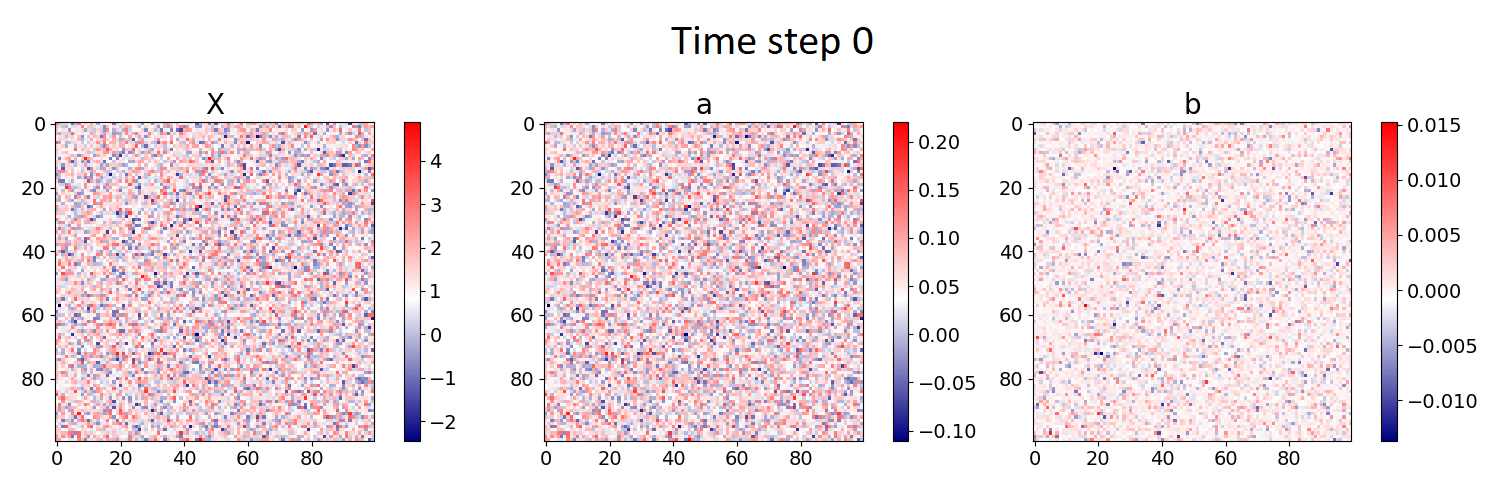
\includegraphics[width=\textwidth]{Flux_composite_00000}\\
	а)
	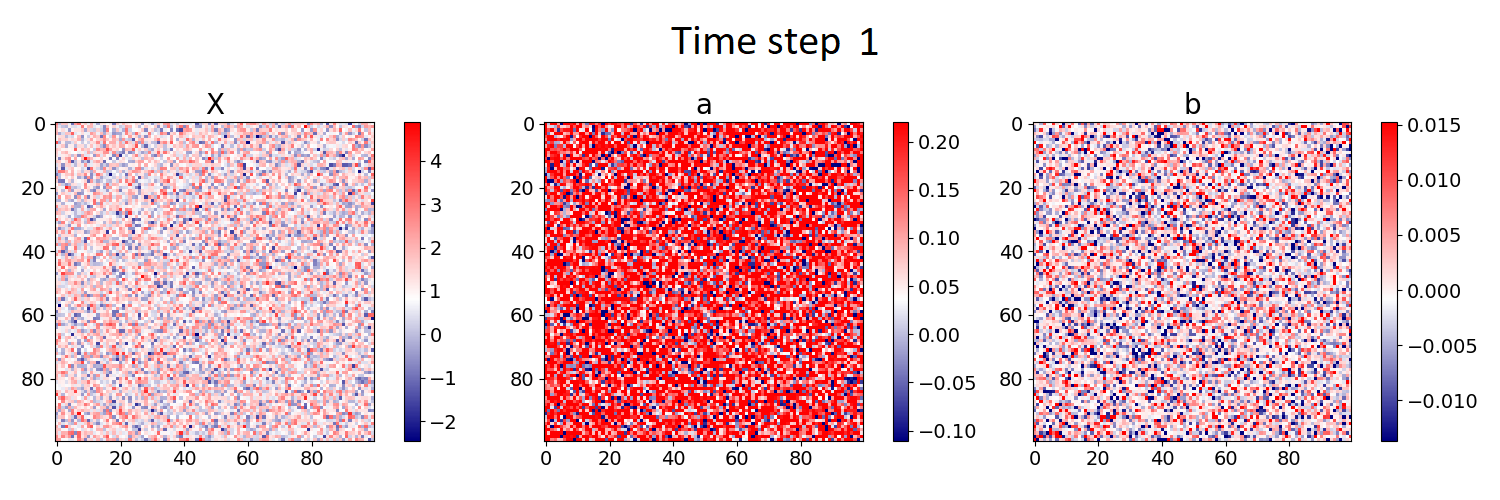
\includegraphics[width=\textwidth]{Flux_composite_00001}\\
	б)
	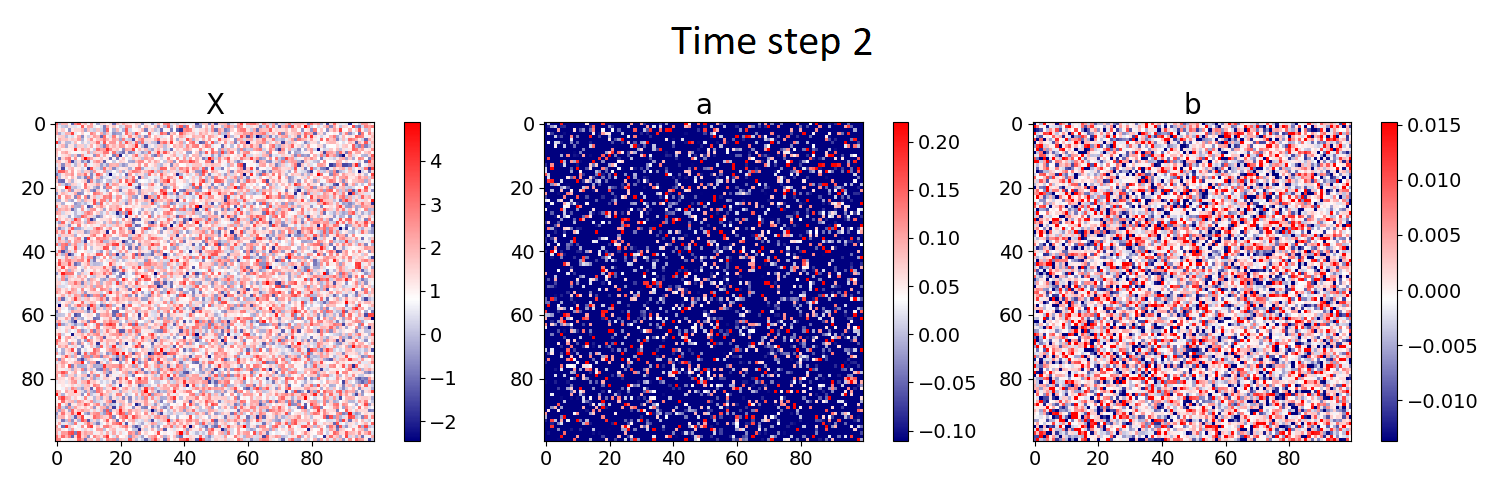
\includegraphics[width=\textwidth]{Flux_composite_00002}\\
	в)
	\caption{Моделируемый процесс $X$ и соответствующие коэффициенты $a$ и $b$ в моменты времени (a) $t=0$, (б) $t=1$, (в) $t=2$}
	\label{fig:flux_simulation}
\end{figure}

На рисунке \ref{fig:flux_simulation} показаны сгенерированные триплеты значений процесса и соответствующие коэффициенты $a(t,X)$ и $b(t,X)$ на первых трех последовательных этапах моделирования матриц размером $100 \times 100$. Оба метода, описанные в разделе 2, применяются к построенному процессу, и полученные в результате оценки коэффициентов сравниваются с заранее заданными функциями $a(t,X)$ и $b(t,X)$.

\begin{figure}[!h]
	\centering
	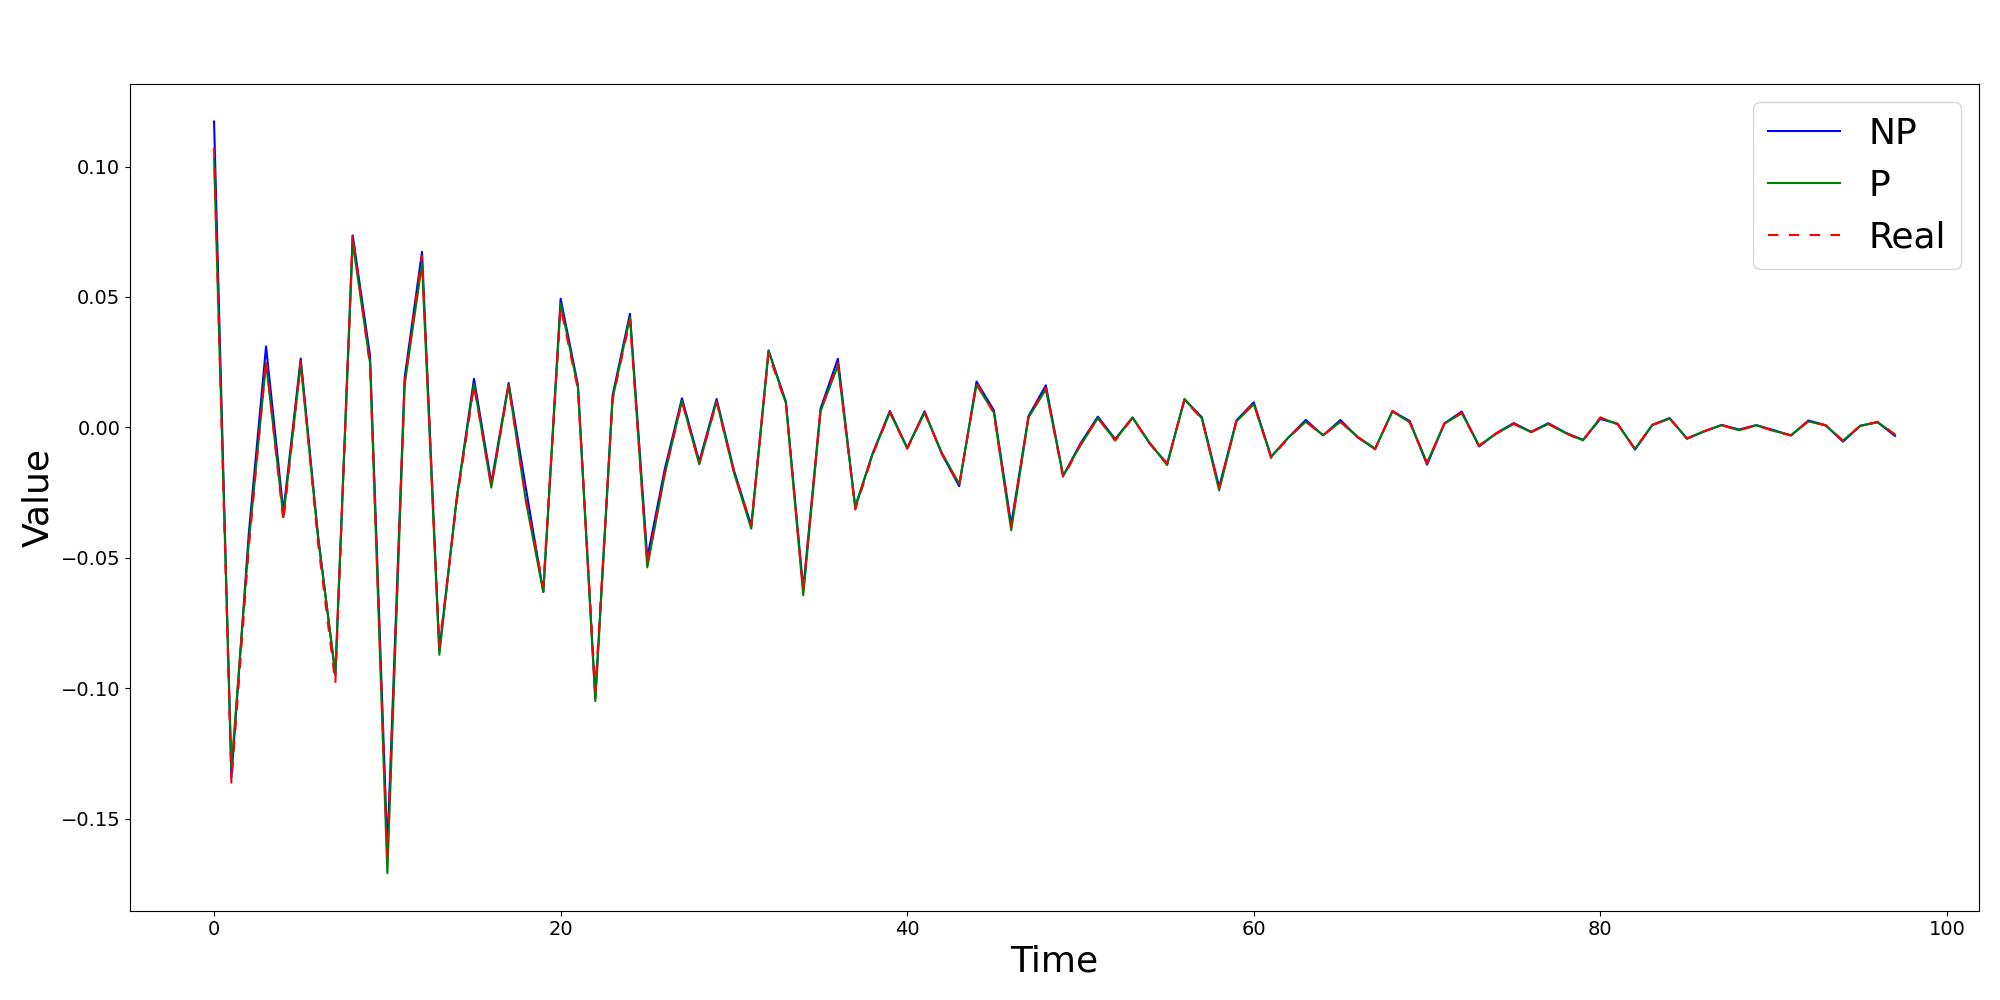
\includegraphics[width=\textwidth]{A_difference_point_(0, 4)-A}\\
	а)
	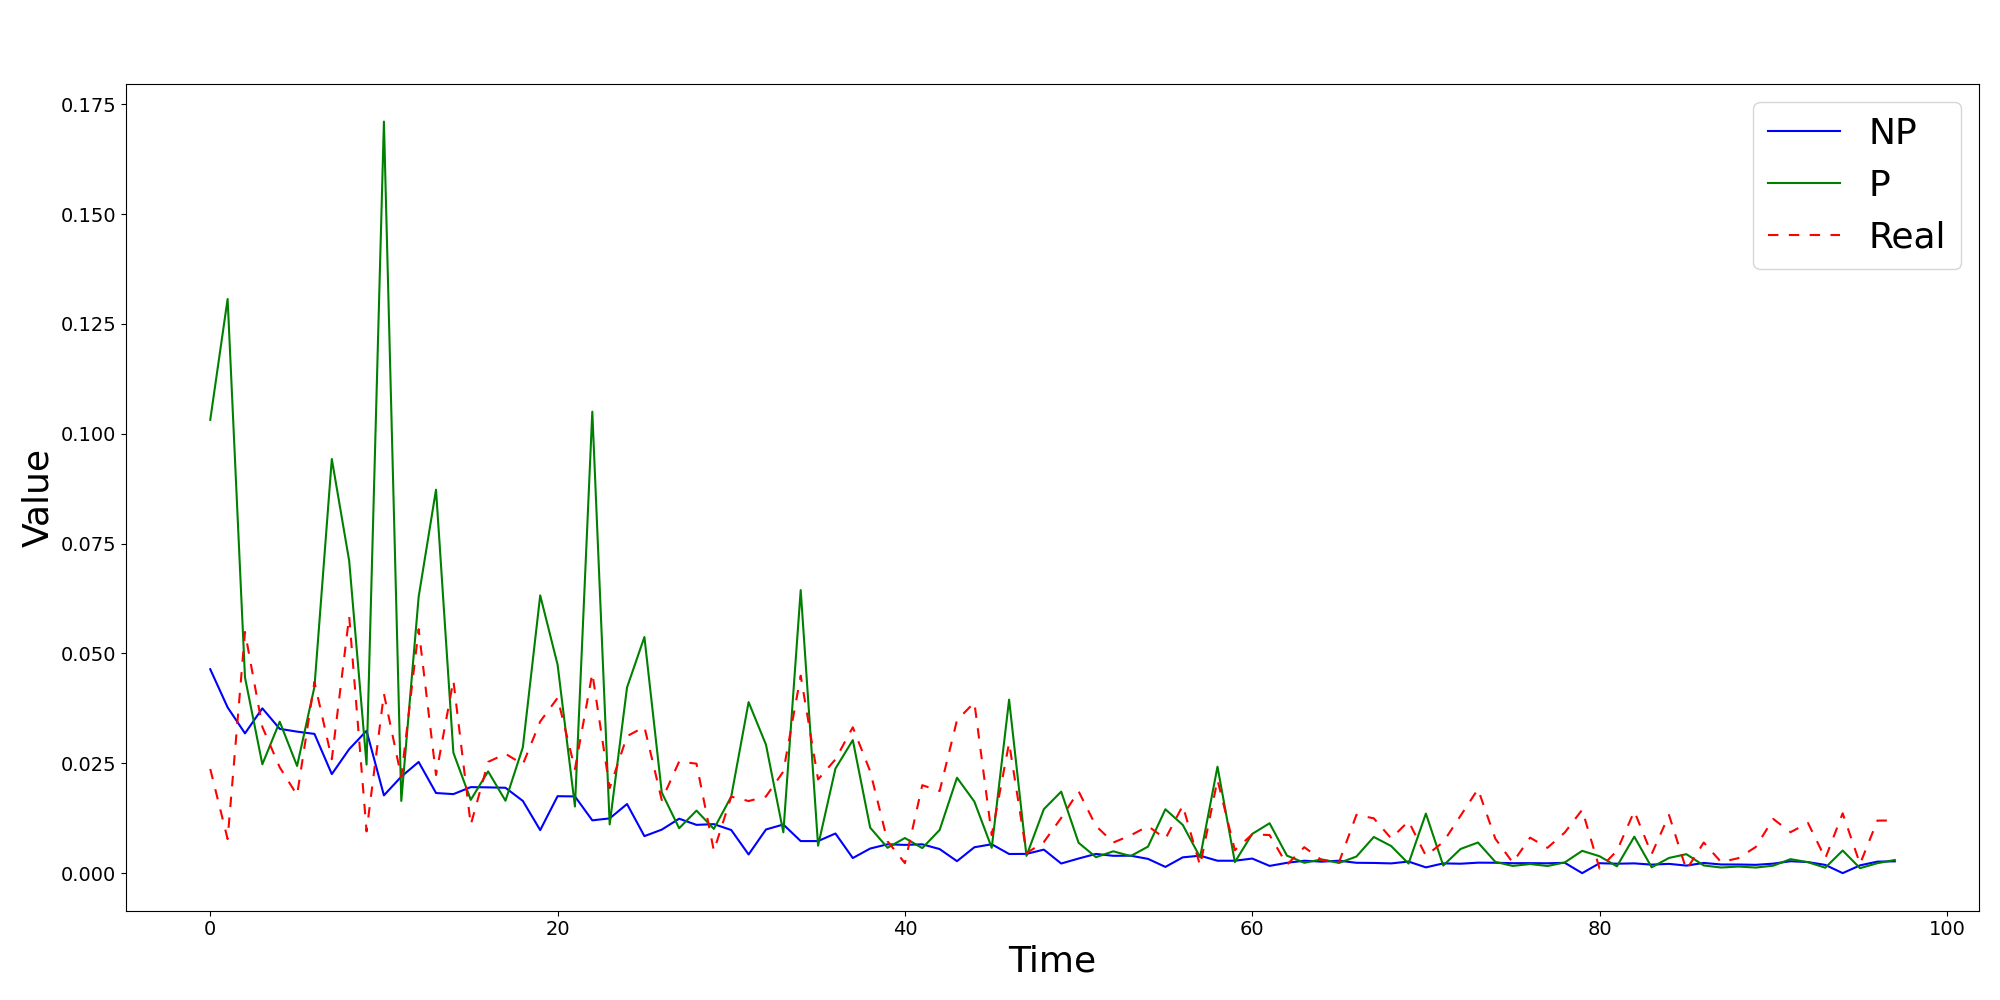
\includegraphics[width=\textwidth]{B_difference_point_(0, 4)-B}\\
	б)
	\caption{Сравнение полученных оценок коэффициентов $a(t,X)$ (а) и $b(t,X)$ (б) непараметрическим (NP) и полупараметрическим (P) методами с реальными значениями в точке $(0,4)$}
	\label{fig:difference_0_4}
\end{figure}

\begin{figure}[!h]
	\centering
	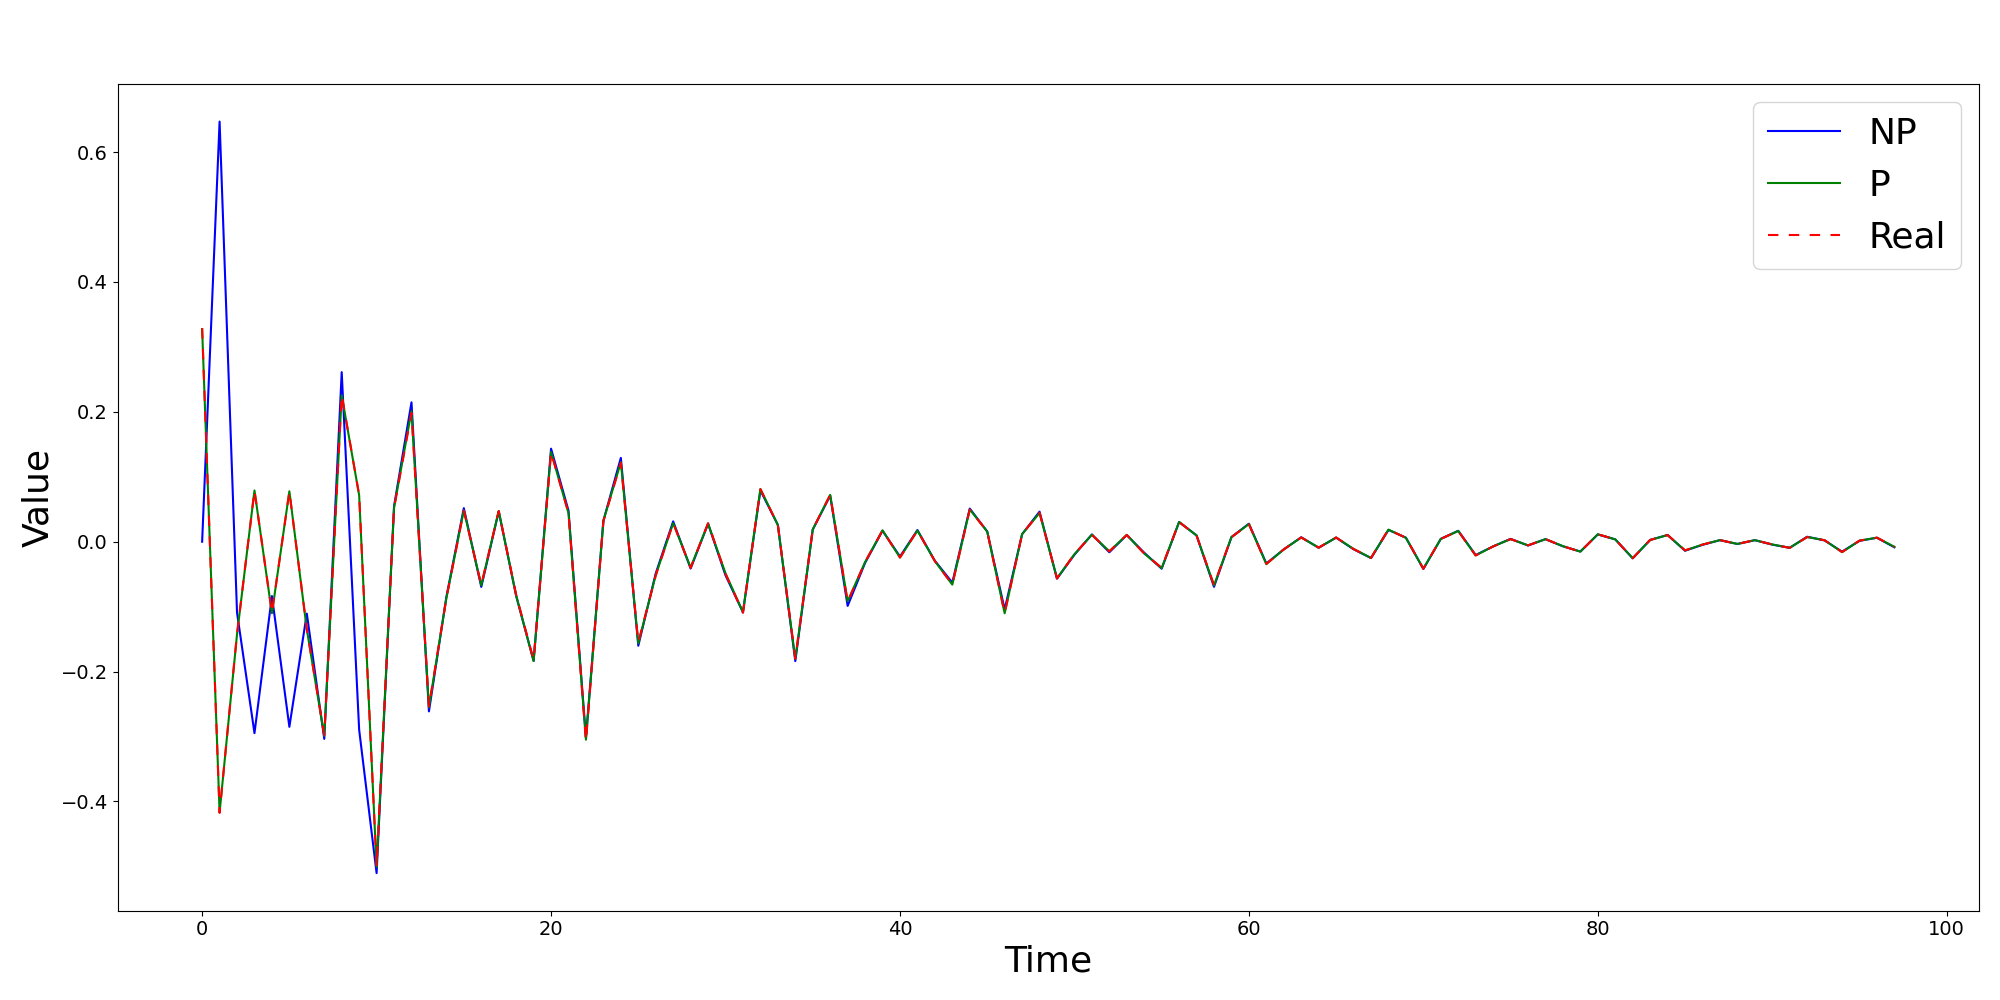
\includegraphics[width=\textwidth]{A_difference_point_(0, 11)-A}\\
	а)
	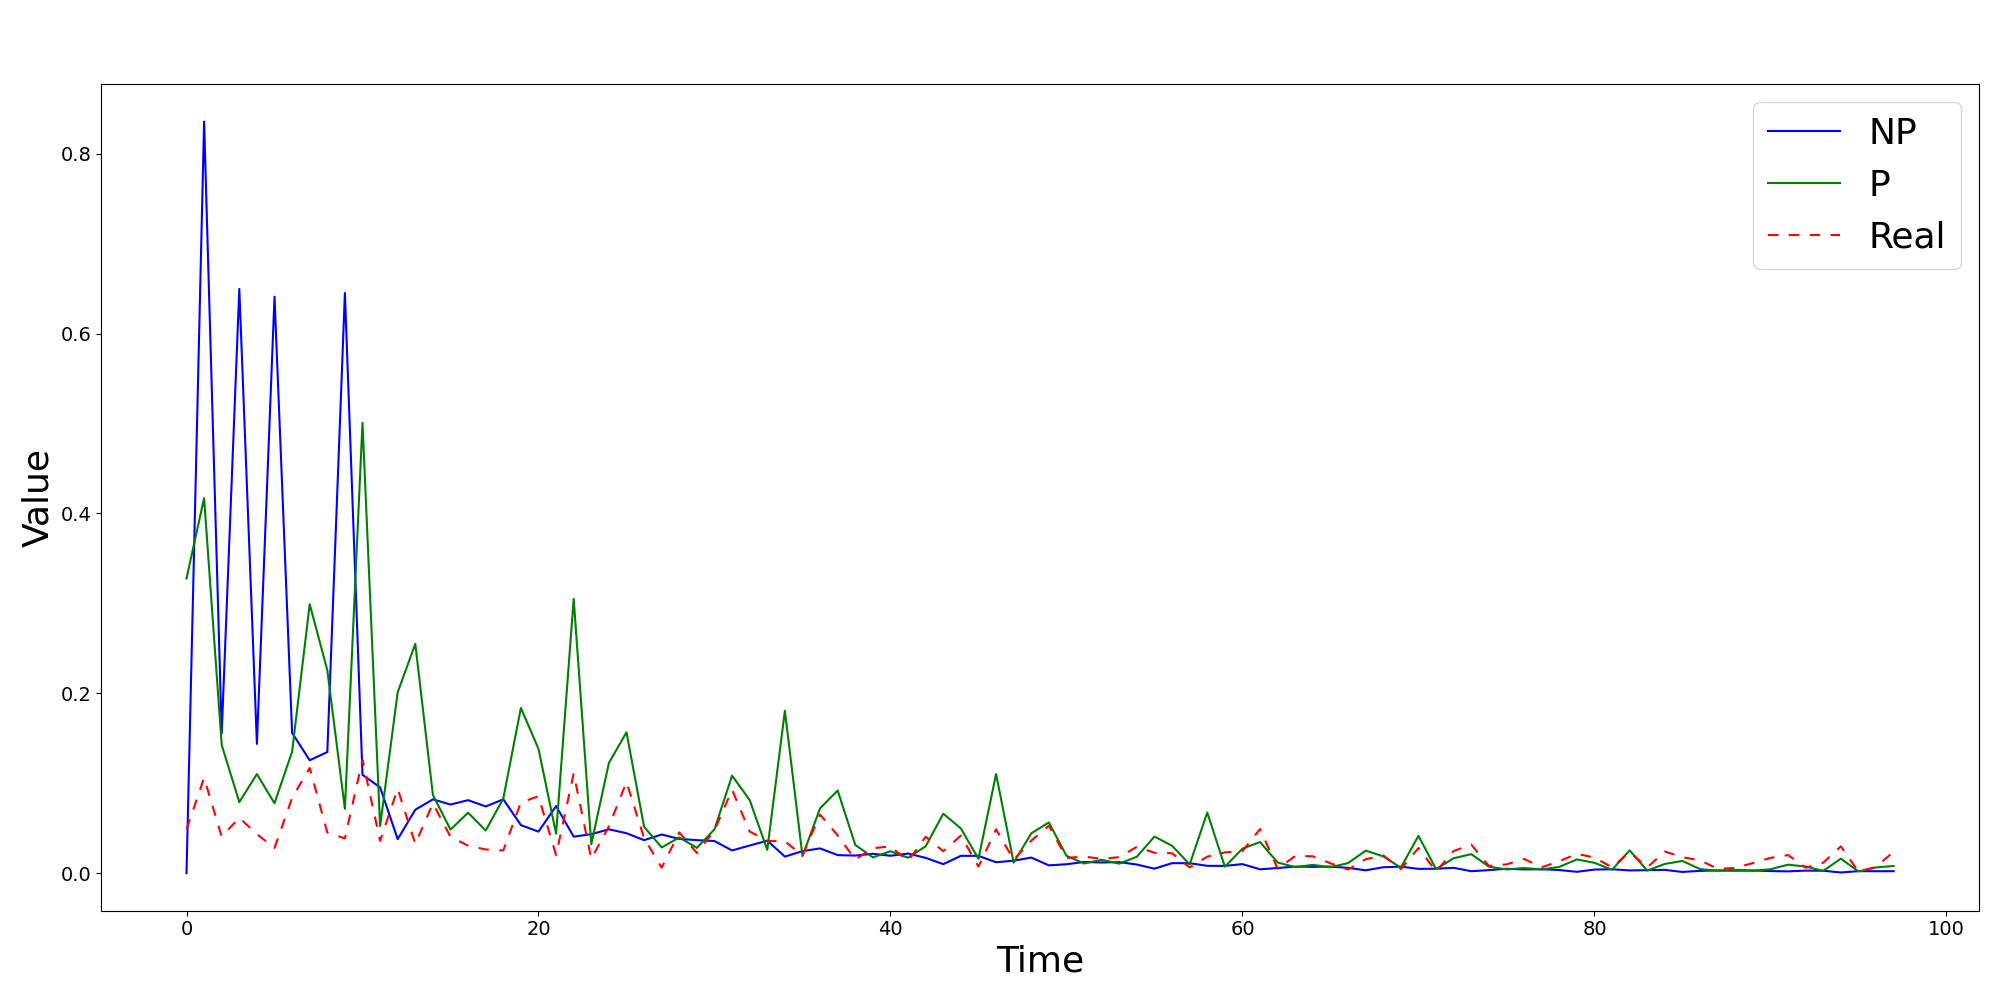
\includegraphics[width=\textwidth]{B_difference_point_(0, 11)-B}\\
	б)
	\caption{Сравнение полученных оценок коэффициентов $a(t,X)$ (а) и $b(t,X)$ (б) непараметрическим (NP) и полупараметрическим (P) методами с реальными значениями в точке $(0,11)$}
	\label{fig:difference_0_11}
\end{figure}

\begin{figure}[!h]
	\centering
	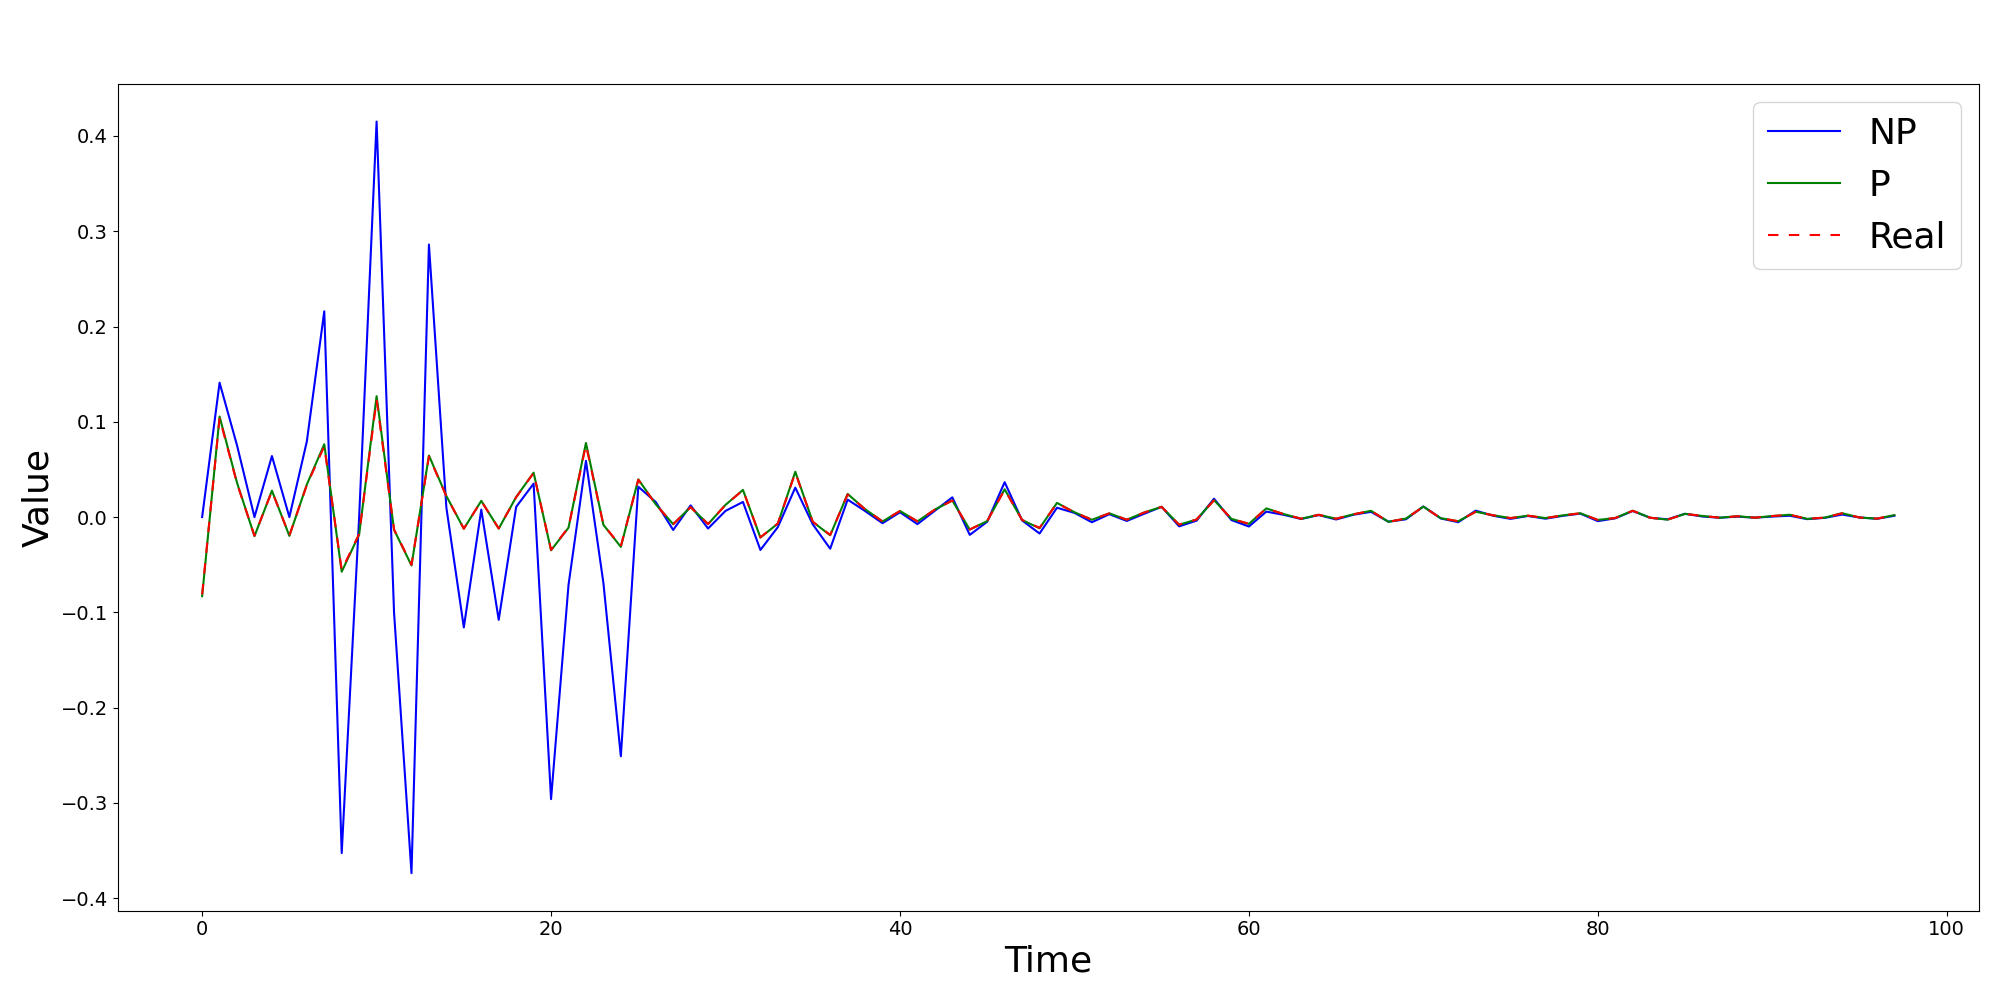
\includegraphics[width=\textwidth]{A_difference_point_(0, 27)-A}\\
	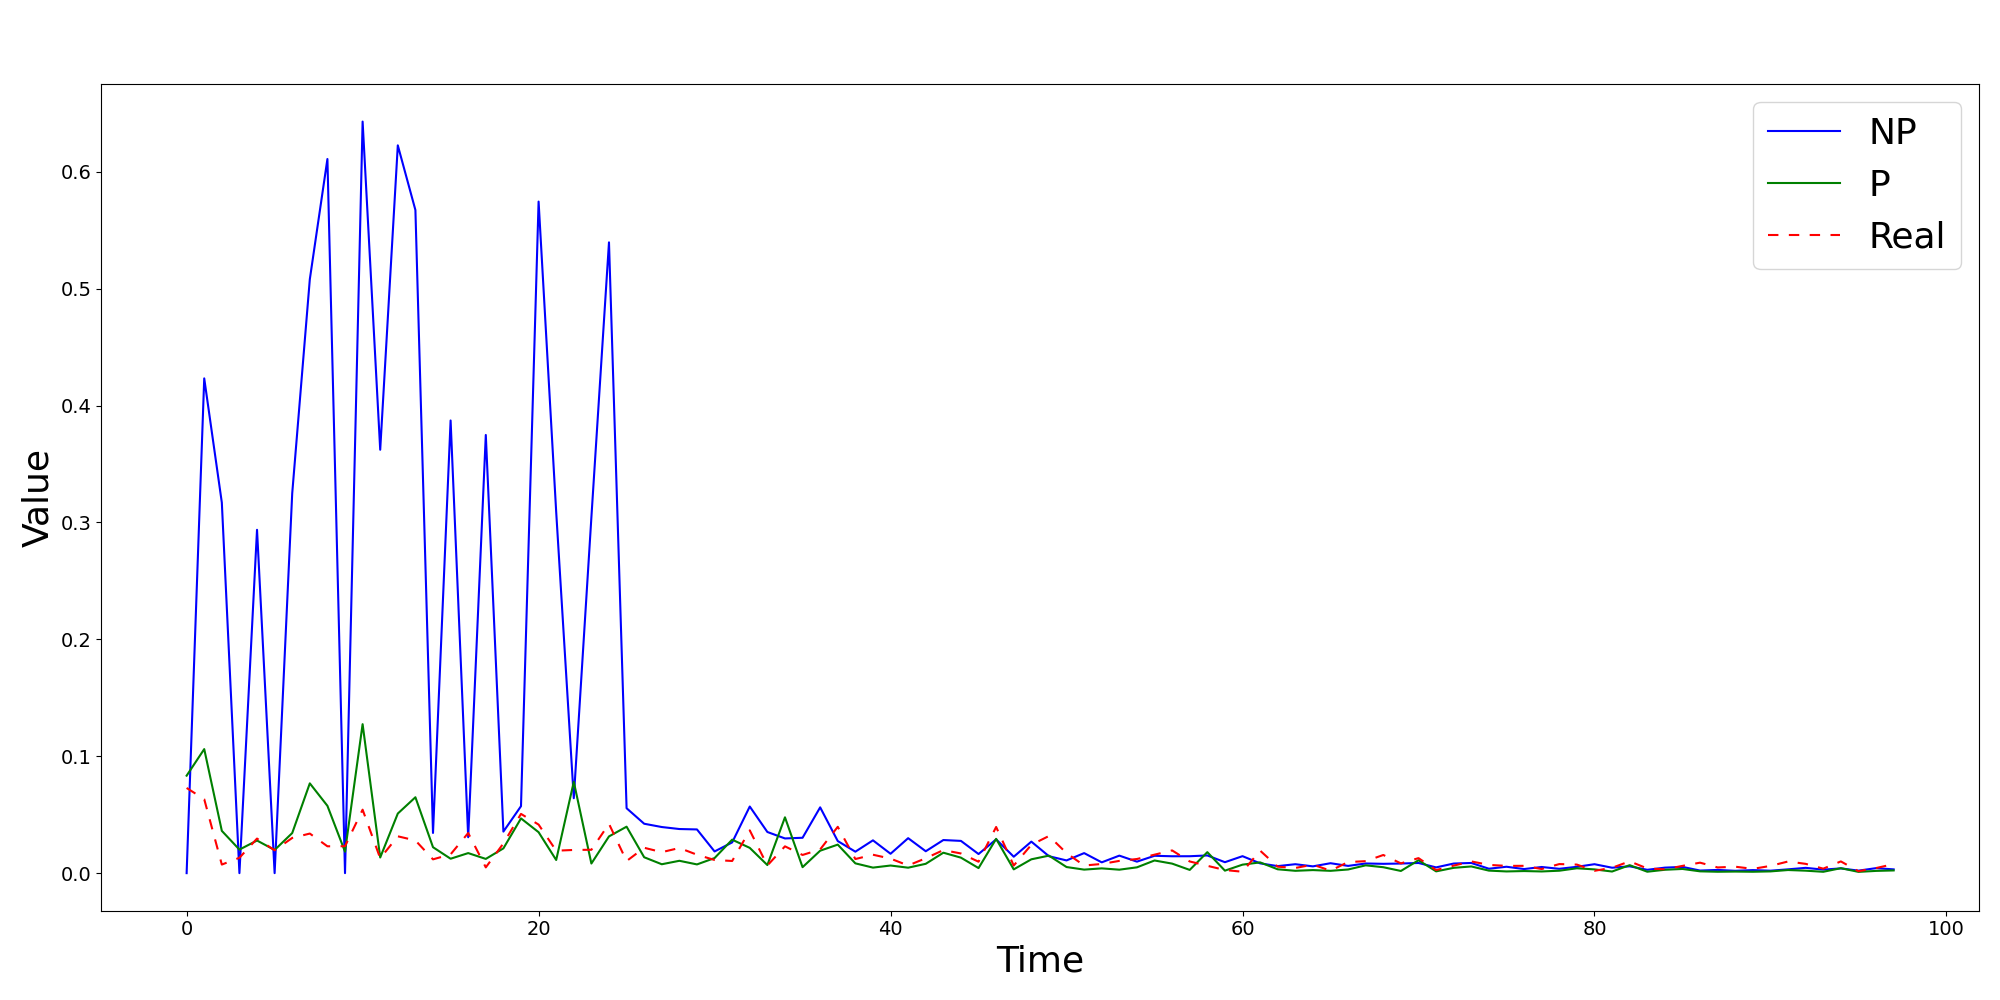
\includegraphics[width=\textwidth]{B_difference_point_(0, 27)-B}\\
	\caption{Сравнение полученных оценок коэффициентов $a(t,X)$ (а) и $b(t,X)$ (б) непараметрическим (NP) и полупараметрическим (P) методами с реальными значениями в точке $(0,27)$}
	\label{fig:difference_0_27}
\end{figure}

На рисунках \ref{fig:difference_0_4}--\ref{fig:difference_0_27} показана эволюция целевых функций с шагом во времени и соответствующие оценки, полученные обоими методами в некоторых фиксированных точках матрицы (узлах сетки), демонстрирующие особенности обоих методов оценки. Ось времени показывает количество шагов генерации. Данные аналогичны показанным на рис. \ref{fig:flux_simulation}, но за гораздо более длительный период времени (около $100$ итераций).
На рисунке \ref{fig:difference_0_4} показан случай, в котором полупараметрический метод уступает непараметрическому с точки зрения RMSE, но гораздо лучше отражает поведение коэффициента диффузии. На рисунке \ref{fig:difference_0_11} показана ситуация, в которой на первых этапах оба метода существенно отличаются от истинного значения коэффициента диффузии $b(t,X)$, но в последующие моменты времени полупараметрический метод начинает лучше описывать тенденцию, значительно превосходя кусочно-линейный вариант непараметрических оценок. Пример явного превосходства полупараметрического метода показан на рисунке \ref{fig:difference_0_27}.

\begin{table}[h!]
	\centering
	\caption{Ошибки в оценках коэффициента $a(t,X)$ полупараметрическим и непараметрическим методами}
	\begin{tabular}{|c|c|c|}
		\hline
		Координаты точки & Полупараметрический метод & Непараметрический метод \\
		\hline
		$(0, 4)$ & $0.02$ & $0.01$ \\
		$(0, 11)$ & $1.28$ & $0.01$ \\
		$(0, 27)$ & $0.72$ & $0.01$ \\
		\hline
	\end{tabular}
	\label{tab:errors_estimation_a}
\end{table}

\begin{table}[h!]
	\centering
	\caption{Ошибки в оценках коэффициента $b(t,X)$ полупараметрическим и непараметрическим методами}
	\begin{tabular}{|c|c|c|}
		\hline
		Координаты точки & Полупараметрический метод & Непараметрический метод \\
		\hline
		$(0, 4)$ & $0.14$ & $0.24$ \\
		$(0, 11)$ & $1.31$ & $0.75$ \\
		$(0, 27)$ & $1.75$ & $0.15$ \\
		\hline
	\end{tabular}
	\label{tab:errors_estimation_b}
\end{table}

В таблицах \ref{tab:errors_estimation_a} и \ref{tab:errors_estimation_b} представлены RMSE-ошибки оценки коэффициентов с помощью обоих методов.

Стоит отметить, что оценки коэффициента дрейфа $a(t,X)$, полученные обоими методами во всех рассмотренных точках смоделированной карты, намного ближе к реальным значениям целевых функций, чем соответствующие оценки коэффициента диффузии $b(t,X)$ к их объективным значениям.


\begin{figure}[!h]
	\centering
	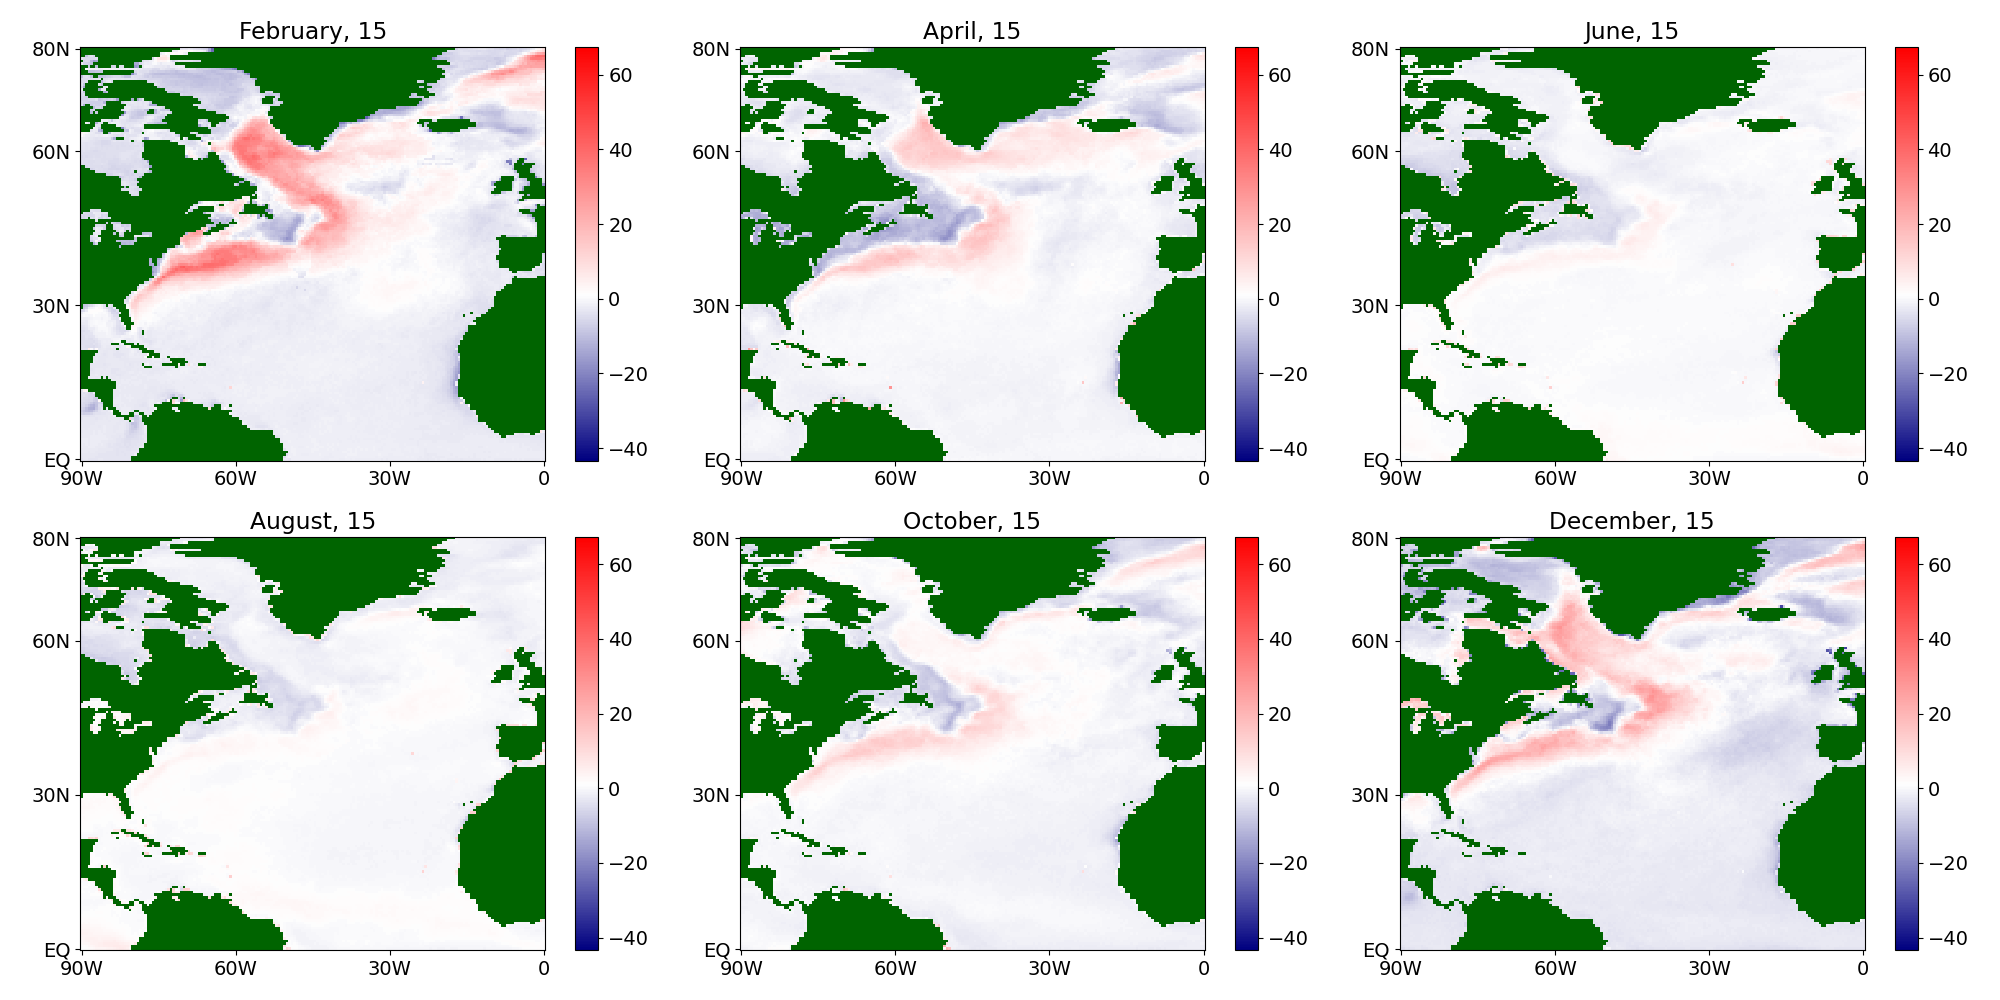
\includegraphics[width=\textwidth]{sensible_a_compare_semiparametric}\\
	а)
	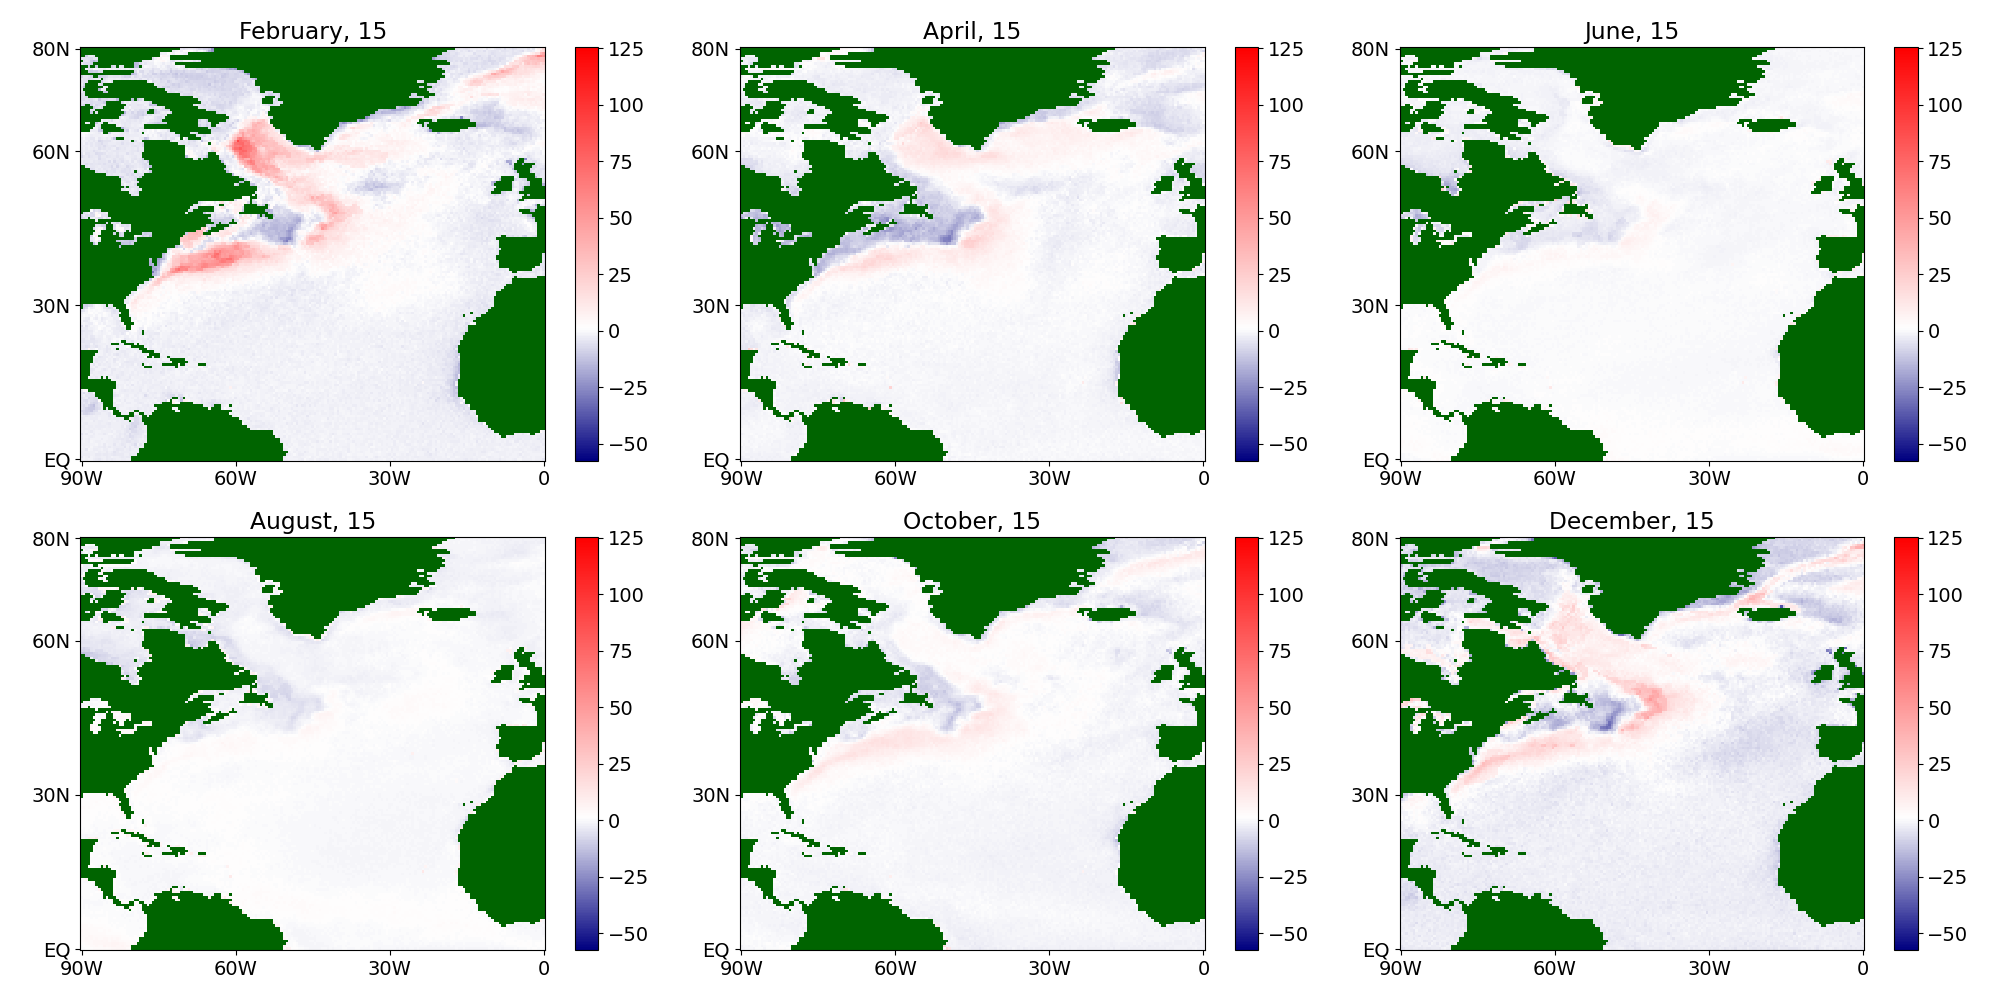
\includegraphics[width=\textwidth]{sensible_a_compare_nonparametric}\\
	б)
	\caption{Оценки коэффициента дрейфа для явного потока в течение среднего года за период $1979-2022$ гг., полученные с помощью (а) полупараметрического метода и (б) непараметрического метода.} 
	\label{fig:sensible_compare_a}
\end{figure}


\begin{figure}[!h]
	\centering
	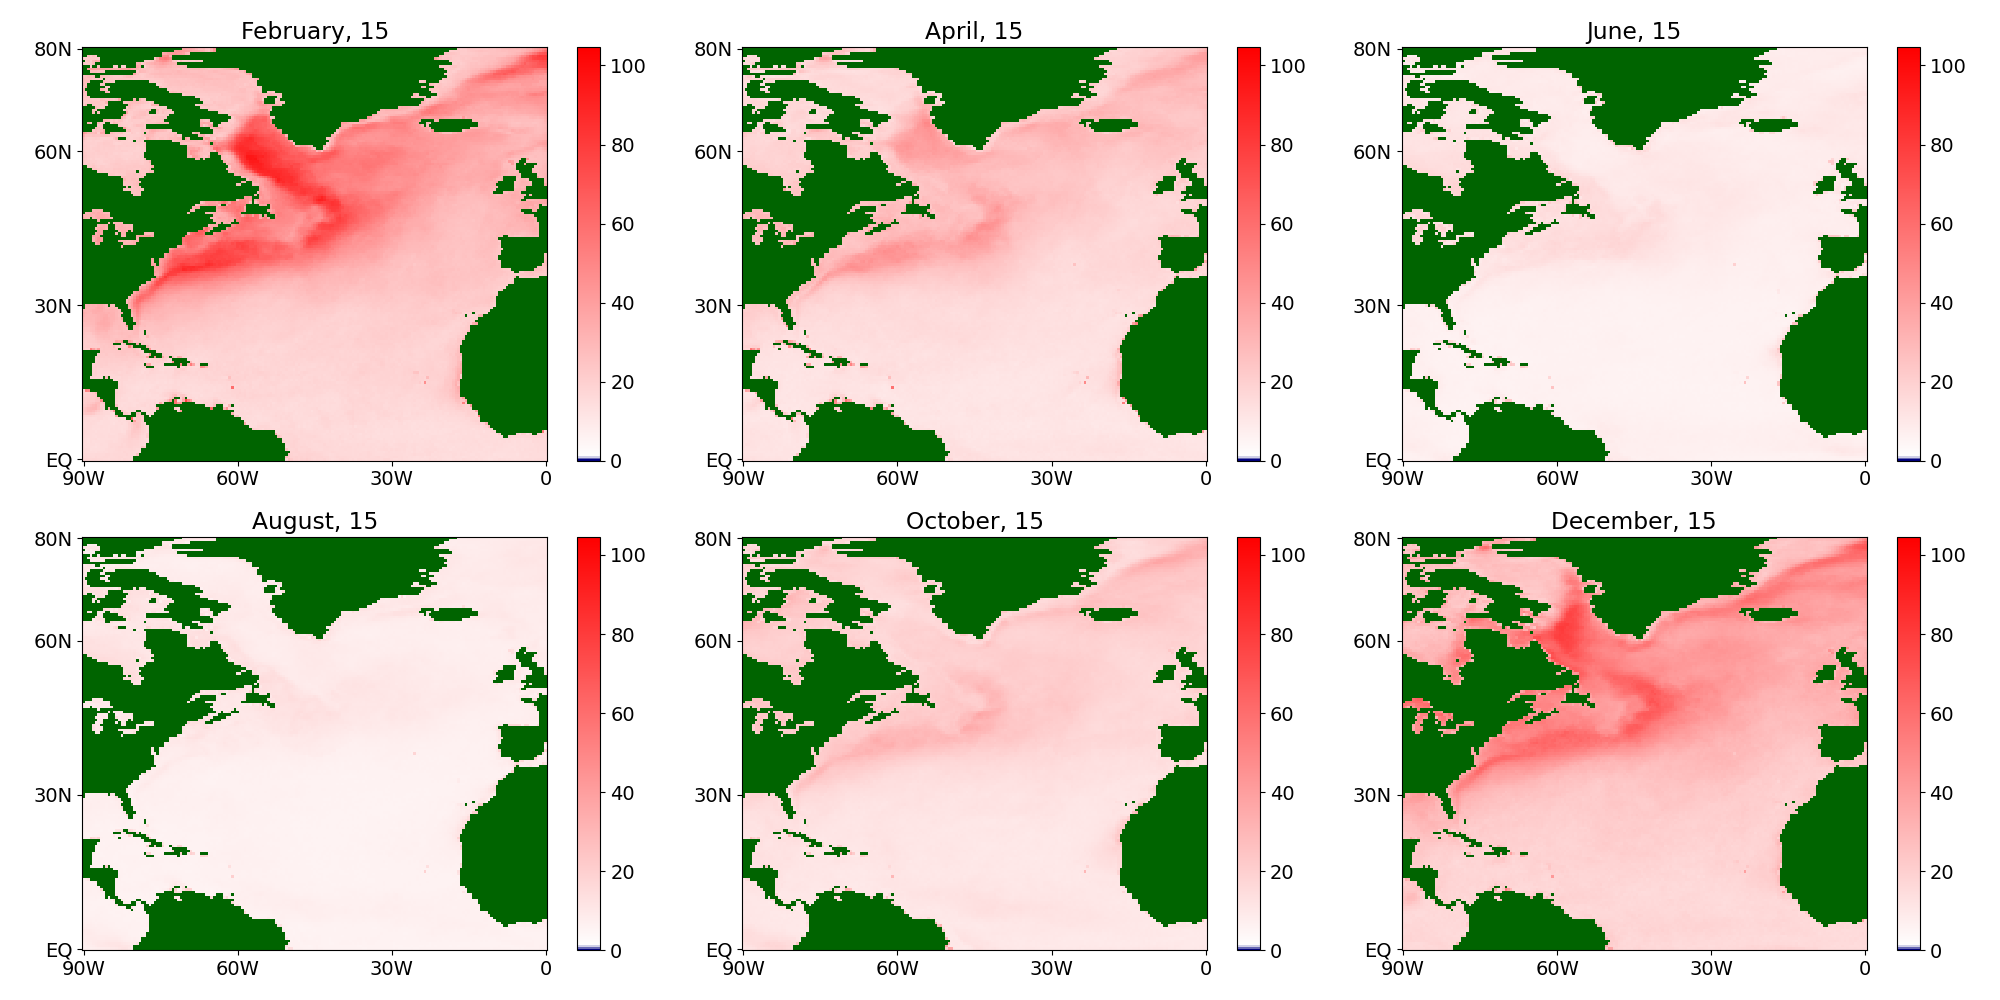
\includegraphics[width=\textwidth]{sensible_b_compare_semiparametric}\\
	а)
	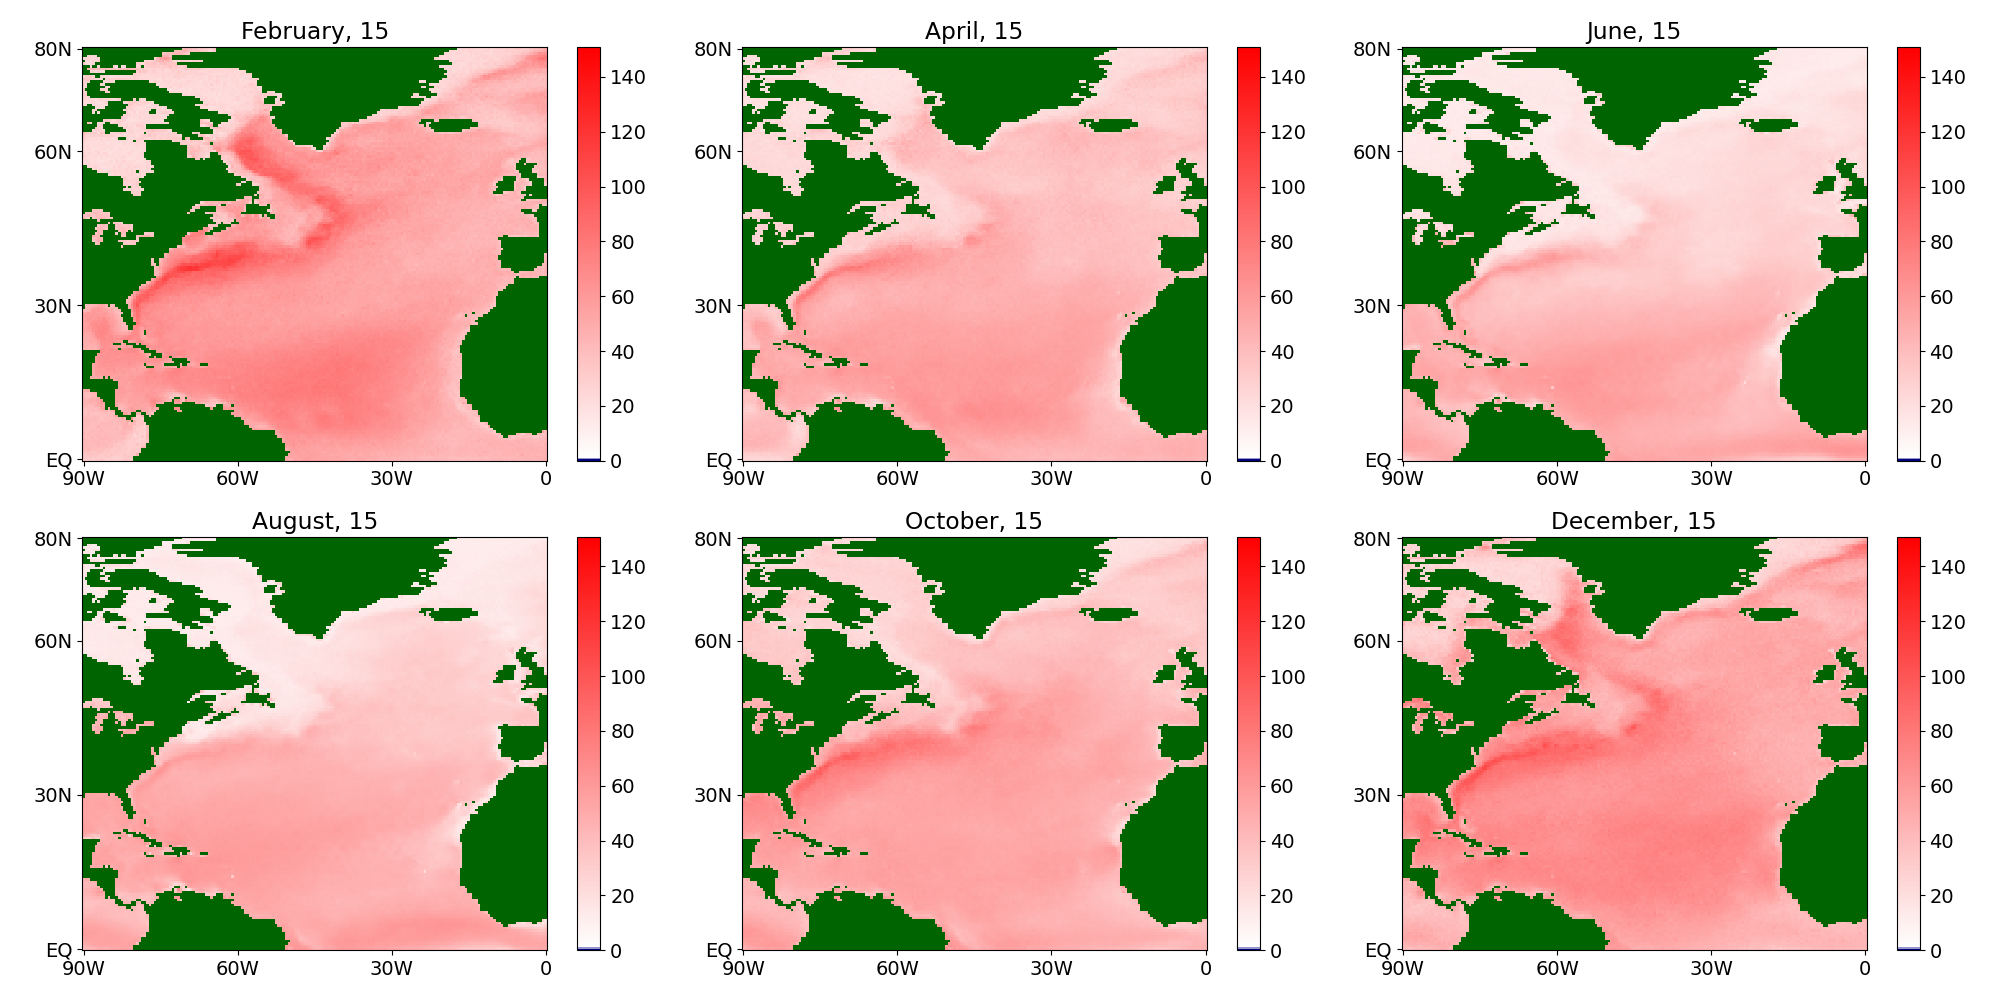
\includegraphics[width=\textwidth]{sensible_b_compare_nonparametric}\\
	б)
	\caption{Оценки коэффициента диффузии для явного потока в течение среднего года за период $1979-2022$ гг., полученные с помощью (а) полупараметрического метода и (б) непараметрического метода.} 
	\label{fig:sensible_compare_b}
\end{figure}

\begin{figure}[!h]
	\centering
	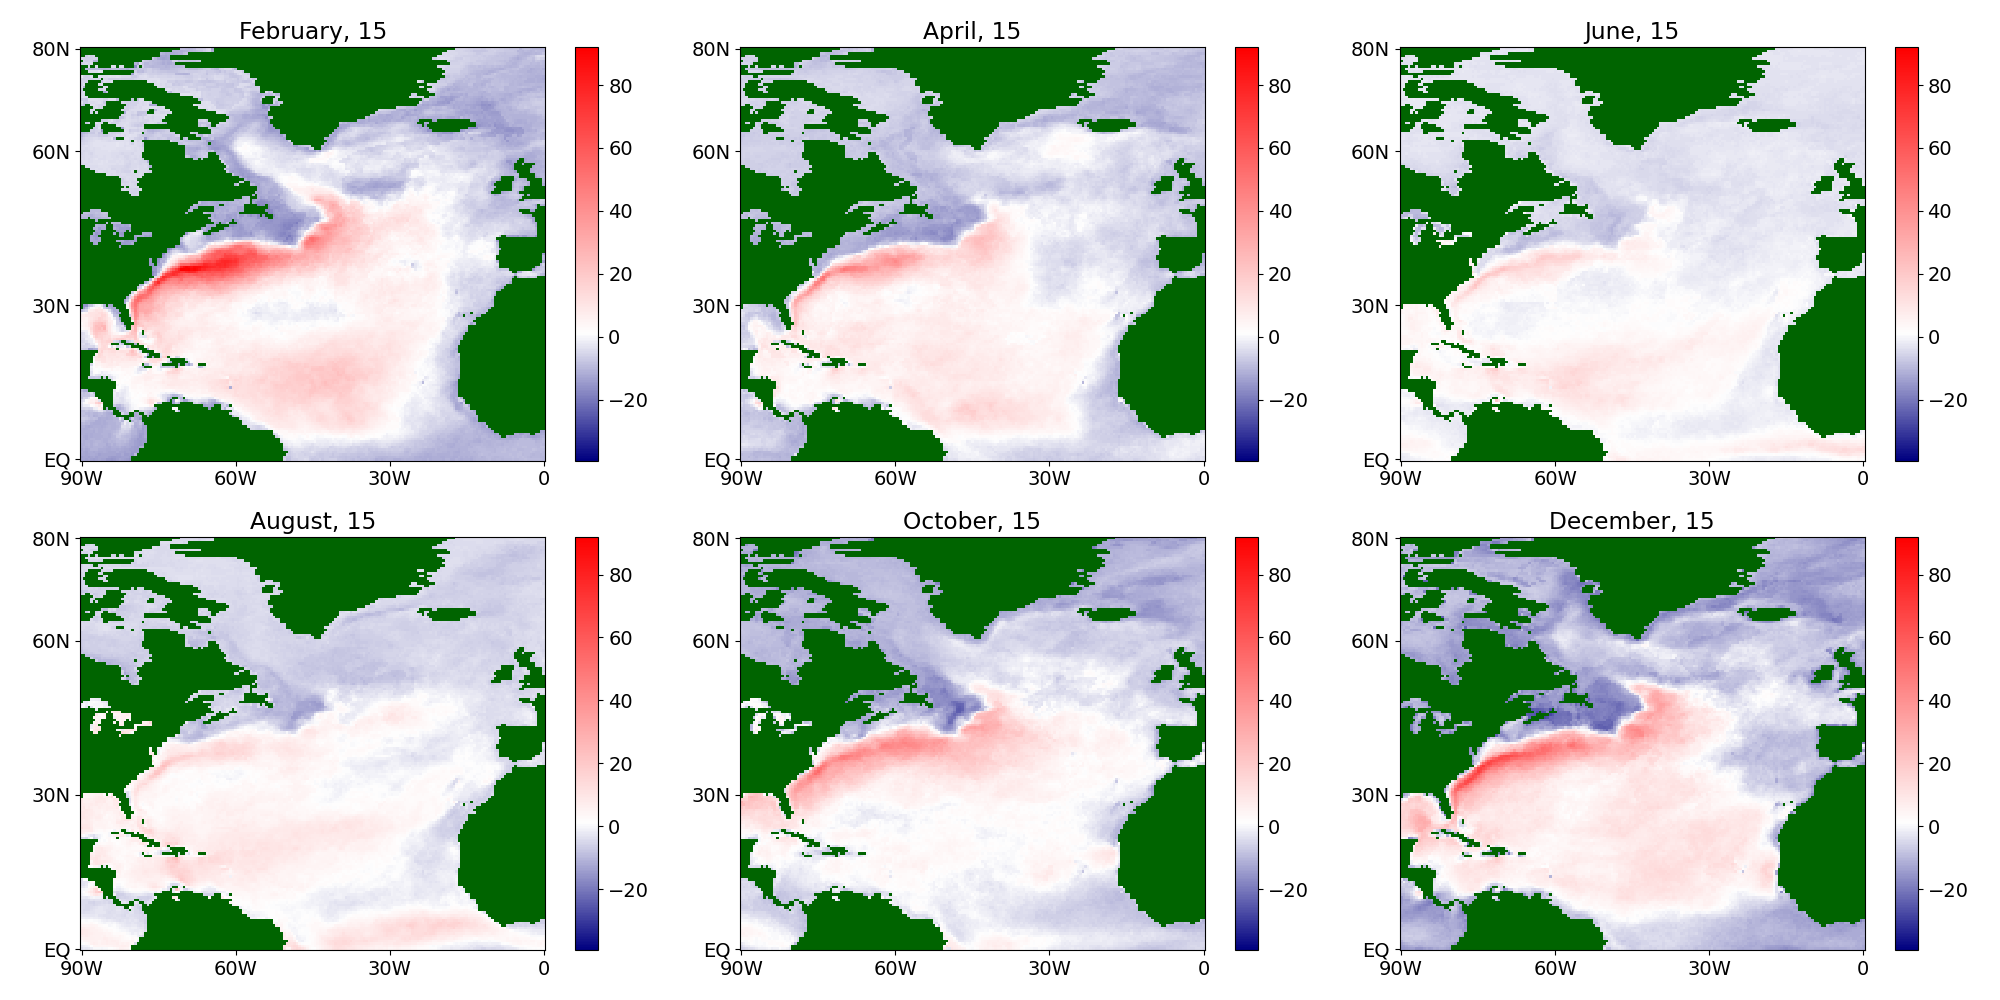
\includegraphics[width=\textwidth]{latent_a_compare_semiparametric}\\
	а)
	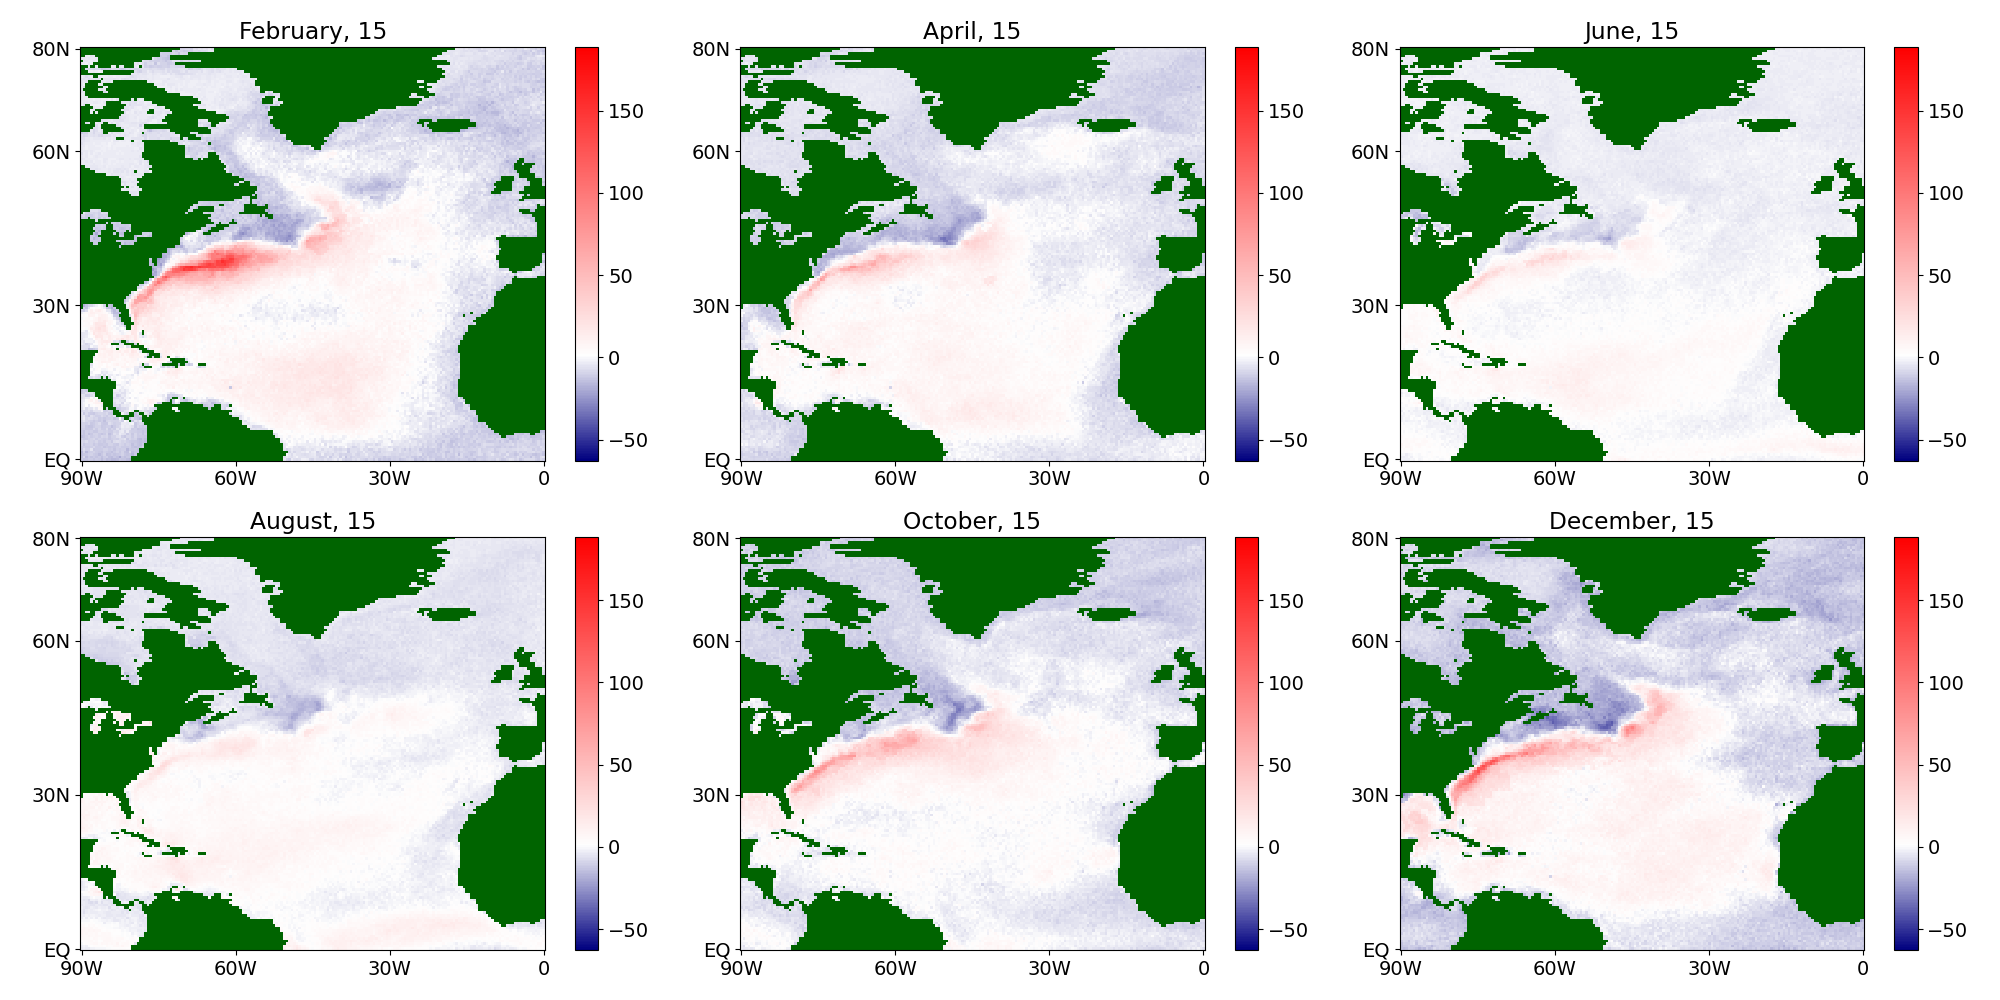
\includegraphics[width=\textwidth]{latent_a_compare_nonparametric}\\
	б)
	\caption{Оценки коэффициента дрейфа для скрытого потока в течение среднего года за период $1979-2022$ гг., полученные с помощью (а) полупараметрического метода и (б) непараметрического метода.} 
	\label{fig:latent_compare_a}
\end{figure}


\begin{figure}[!h]
	\centering
	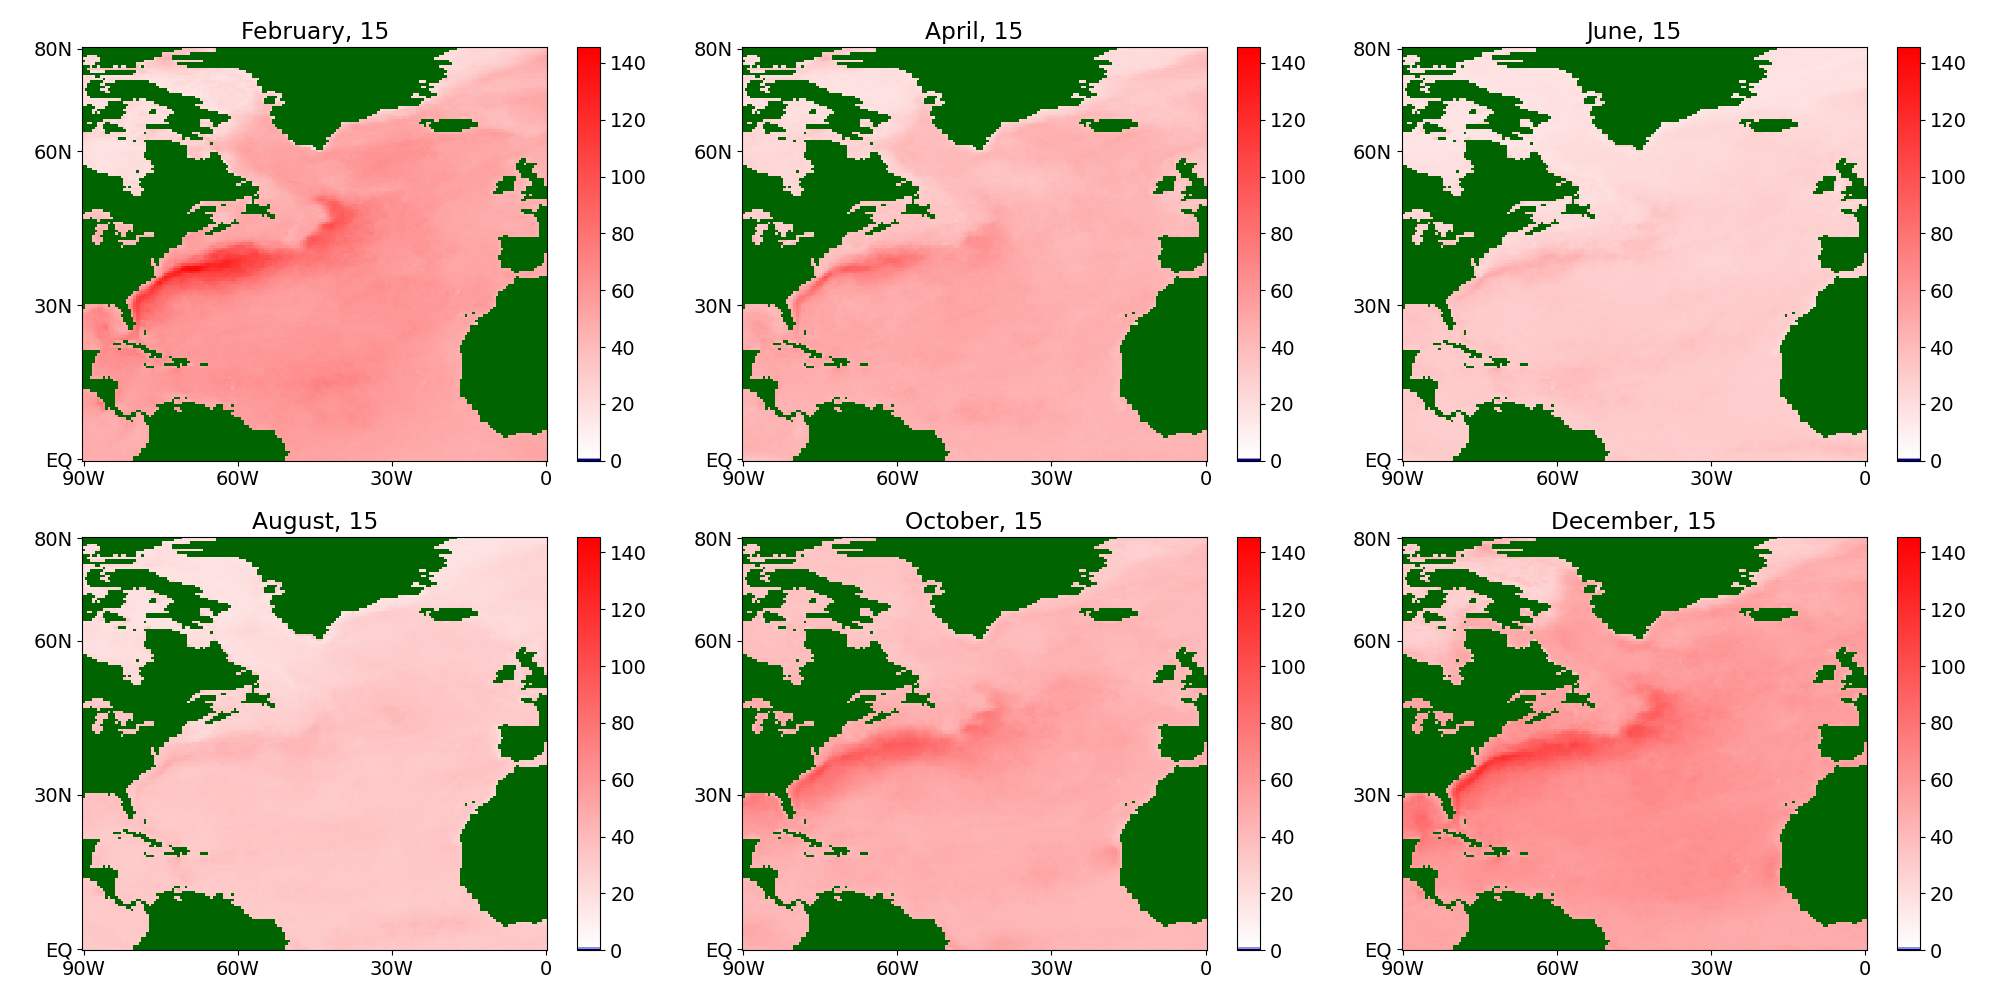
\includegraphics[width=\textwidth]{latent_b_compare_semiparametric}\\
	а)
	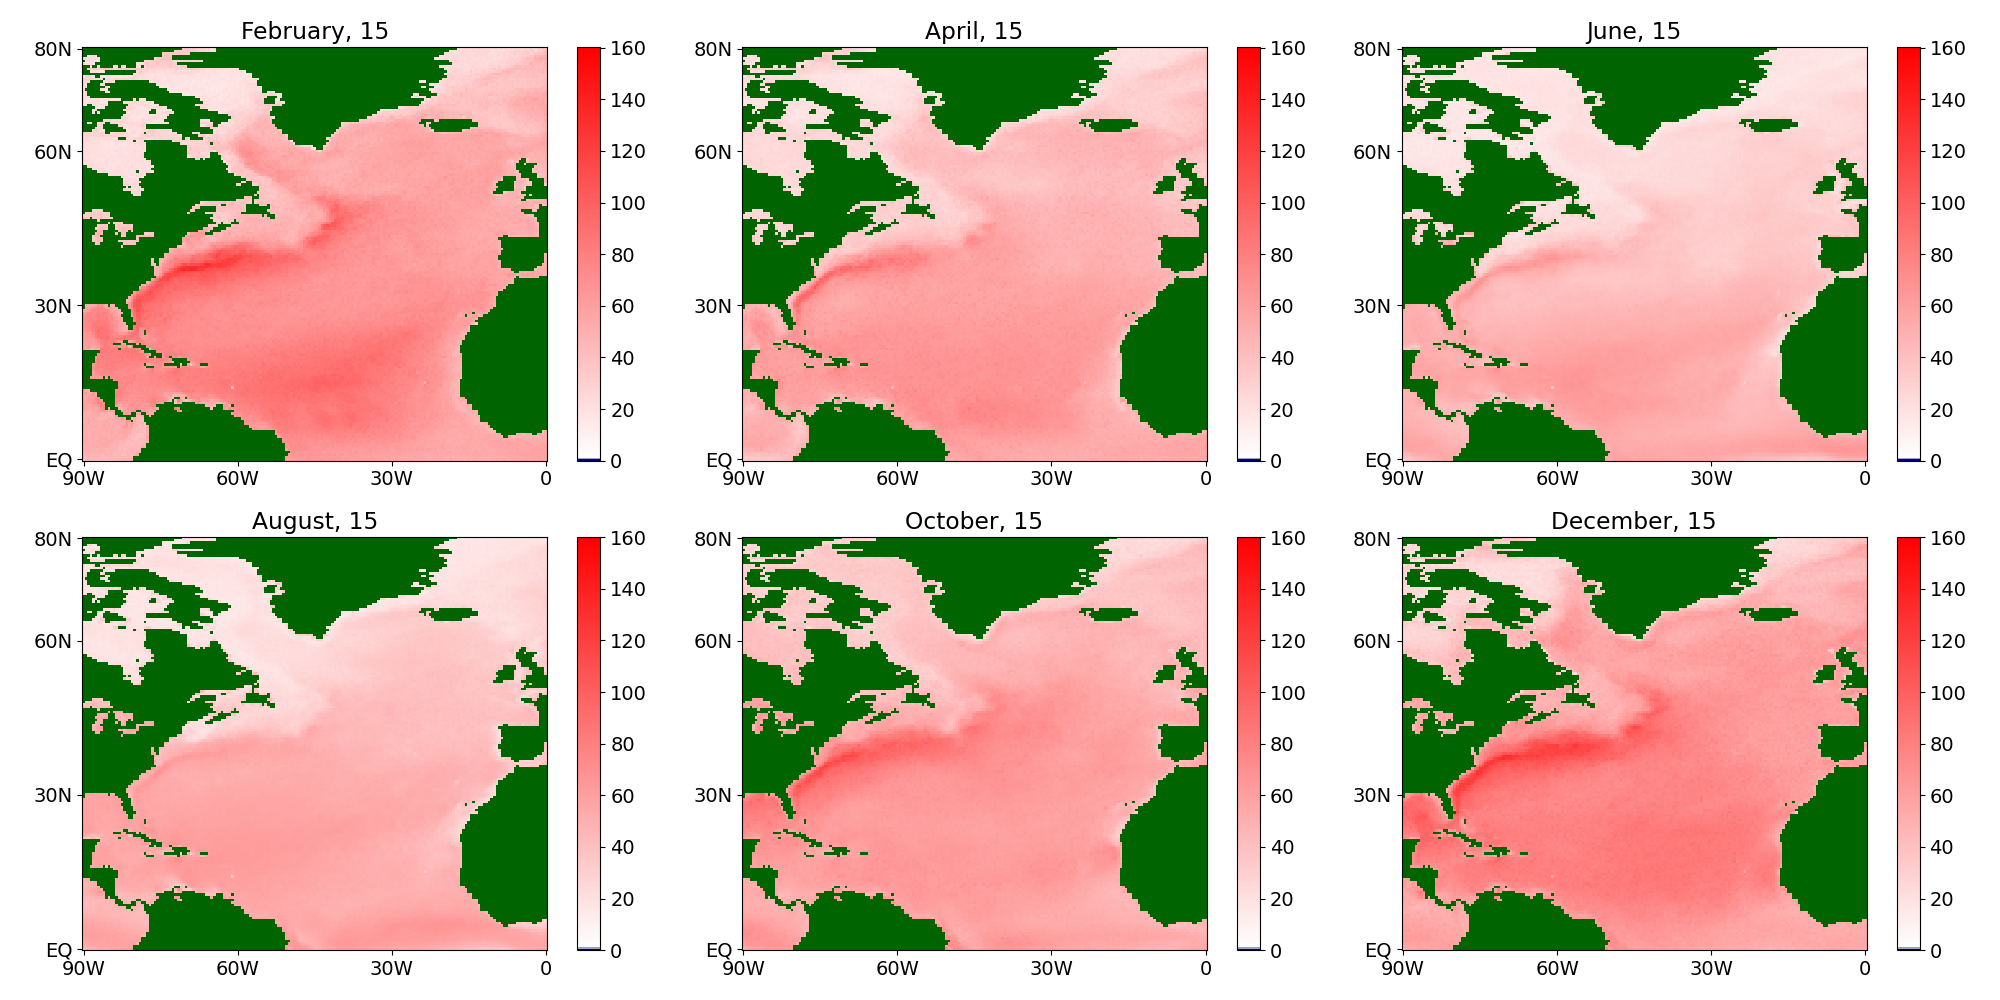
\includegraphics[width=\textwidth]{latent_b_compare_nonparametric}\\
	б)
	\caption{Оценки коэффициента диффузии для скрытого потока в течение среднего года за период $1979-2022$ гг., полученные с помощью (а) полупараметрического метода и (б) непараметрического метода.} 
	\label{fig:latent_compare_b}
\end{figure}

\subsection{Данные реанализа}
В данном разделе оба метода применяются к реальным данным реанализа явного и скрытого потоков тепла в Северной Атлантике за период с $1979$ по $2022$ год, взятых из базы данных ERA5.

На рисунках \ref{fig:sensible_compare_a}-\ref{fig:latent_compare_b} показаны результаты применения обоих методов для данных явных и скрытых тепловых потоков в течение так называемого “среднего года”, которые построены следующим образом: в каждый из шести выбранных фиксированных дней в году в разное время года (а именно, $15$ февраля, $15$ апреля, $15$ июня, $15$ августа, $15$ октября, и $15$ декабря), полученные оценки усредняются по всем рассматриваемым годам. Это позволяет сгладить отдельные выбросы, возникающие как непосредственно в самих данных, так и из-за вычислительных ошибок при расчете точечных оценок. Результаты применения непараметрического метода к тем же данным и их анализ с геофизической точки зрения за этот период можно найти в работе~\cite{gorshenin2023stochastic}.

Цветовая гамма на картах меняется с синего (соответствующего отрицательным значениям) до белый (при значениях, близких к нулю) и далее до красного (соответствующего положительным значениям). Яркость цвета в определенной точке соответствует удаленности значения от нуля. Участки суши выделены темно-зеленым цветом. На картах, соответствующих оценкам коэффициента диффузии, синий цвет не отображается, поскольку значения оценок неотрицательны (с физической точки зрения коэффициент диффузии эквивалентен дисперсии случайной величины).

На рисунке \ref{fig:sensible_compare_a} показан пример значений оценок, полученных с помощью обоих методов, для коэффициента дрейфа явного потока в течение среднего года. Видно, что визуально оба метода сильно совпадают, но оценки, полученные полупараметрическим методом, более плавно меняют цвет в соседних узлах карты (то есть имеют более близкие значения), а также имеют значения в областях пиков в абсолютном смысле меньше, чем соответствующие оценки, полученные с помощью непараметрического метода. Географическое расположение максимальных абсолютных значений, как и ожидалось, хорошо соответствует зонам сильных струйных течений в Северной Атлантике. Также наблюдается сезонный цикл: в зимние месяцы коэффициент дрейфа положительный, тогда как в летние месяцы он отрицательный.

Локализация, полученная с помощью непараметрического метода, является более грубой и менее детализированной, чем полученная с помощью полупараметрического метода. Аналогичные выводы справедливы и для коэффициента диффузии (см. рис. \ref{fig:sensible_compare_b}), хотя указанный эффект оказывается менее выраженным. Оценки коэффициента диффузии характеризуются обширными зонами своего максимального значения и менее выраженным сезонным циклом, чем для соответствующего коэффициента дрейфа, хотя в летние месяцы максимум заметно меньше в обоих методах, как для явных, так и для скрытых потоков. На рисунках \ref{fig:latent_compare_a} и \ref{fig:latent_compare_b} представлены оценки коэффициентов для скрытых потоков.

\begin{figure}[!h]
	\centering
	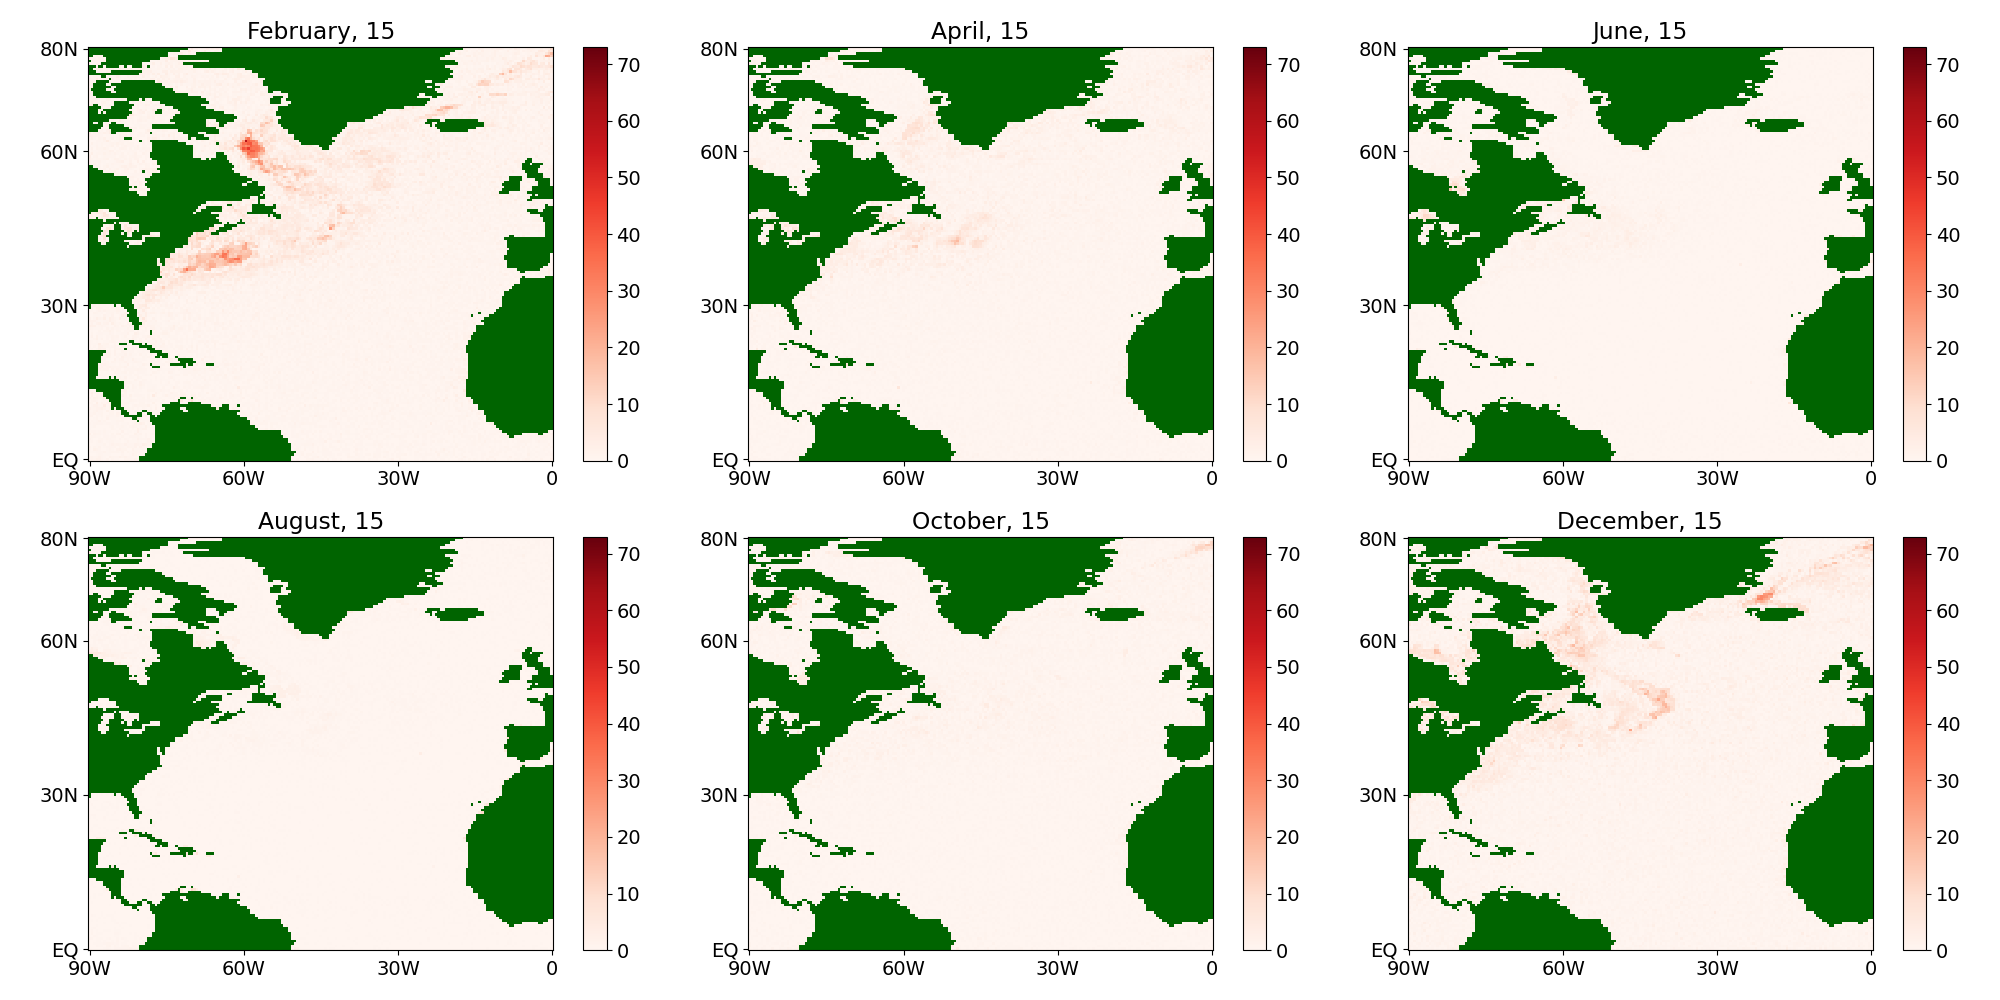
\includegraphics[width=\textwidth]{difference_a_compare_sensible}
	\caption{Абсолютная разность оценок коэффициента дрейфа для явного потока в течение среднего года за период $1979-2022$ гг.} 
	\label{fig:sensible_difference_a}
\end{figure}


\begin{figure}[!h]
	\centering
	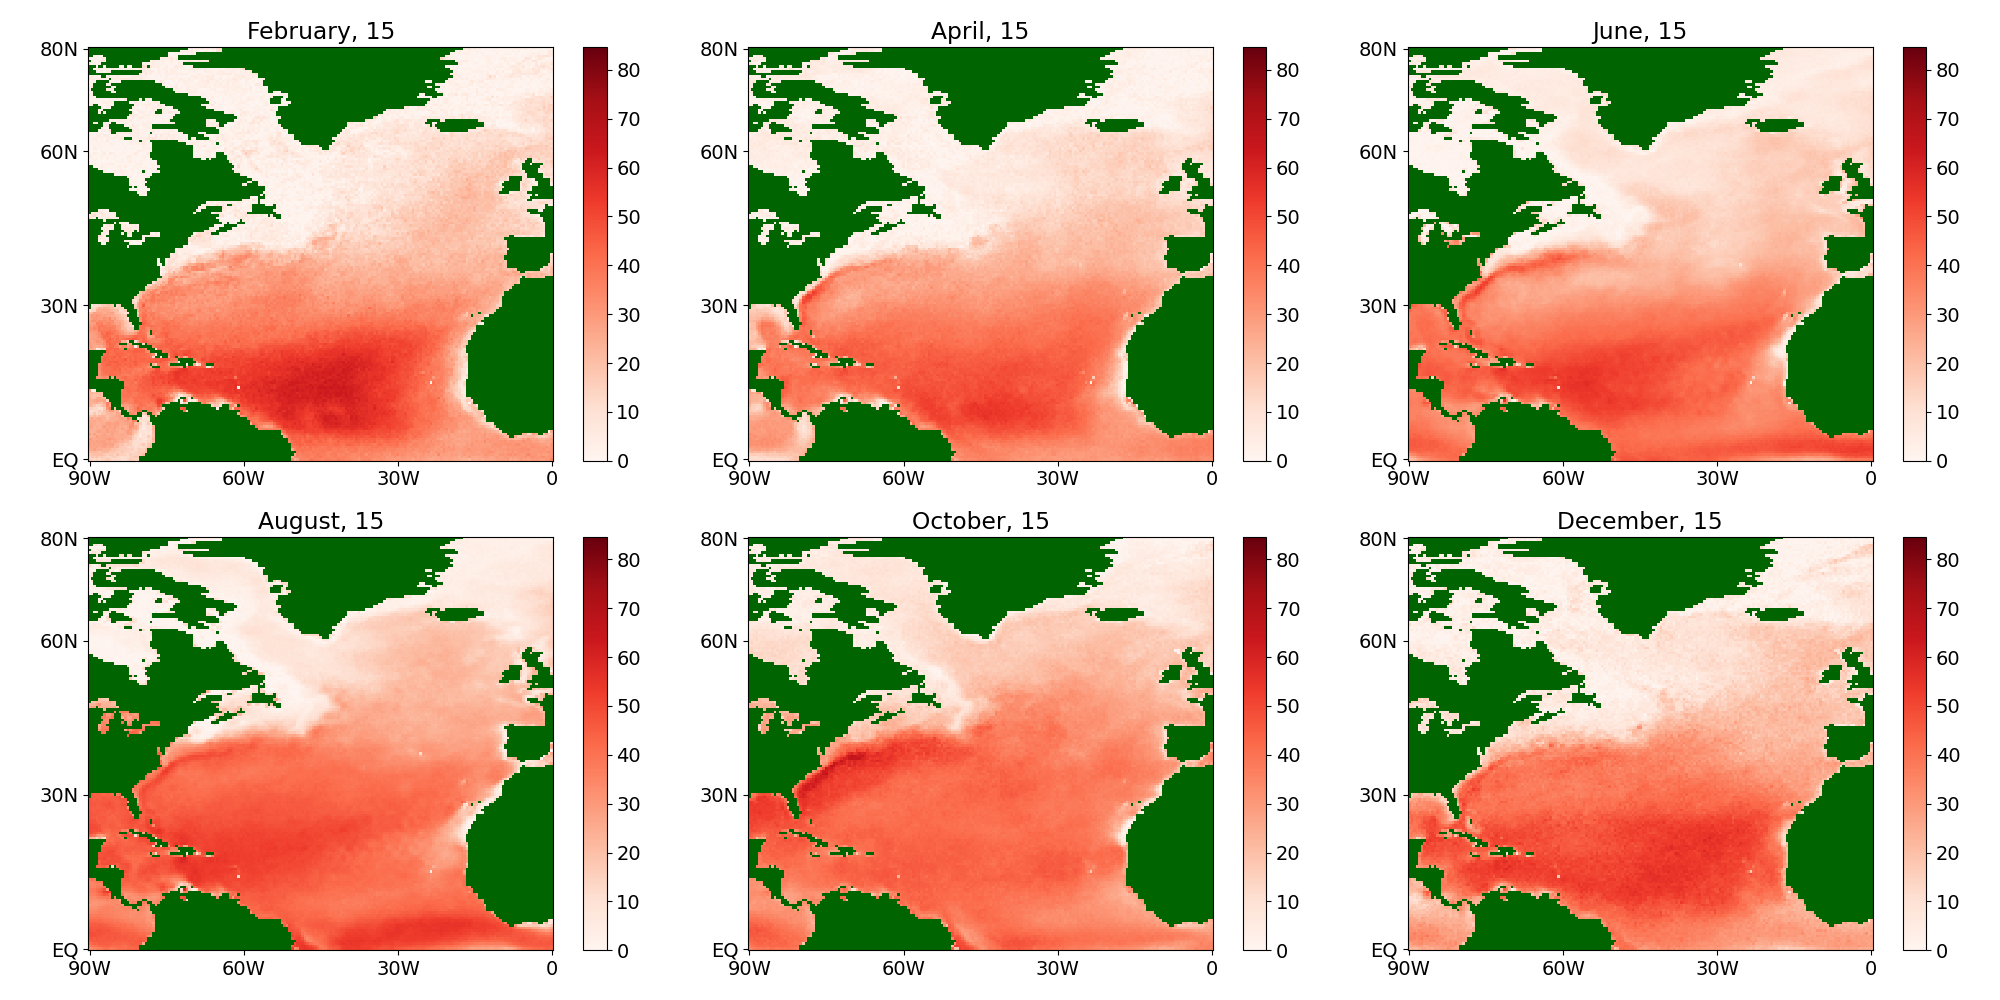
\includegraphics[width=\textwidth]{difference_b_compare_sensible}
	\caption{Абсолютная разность оценок коэффициента диффузии для явного потока в течение среднего года за период $1979-2022$ гг.} 
	\label{fig:sensible_difference_b}
\end{figure}

\begin{figure}[!h]
	\centering
	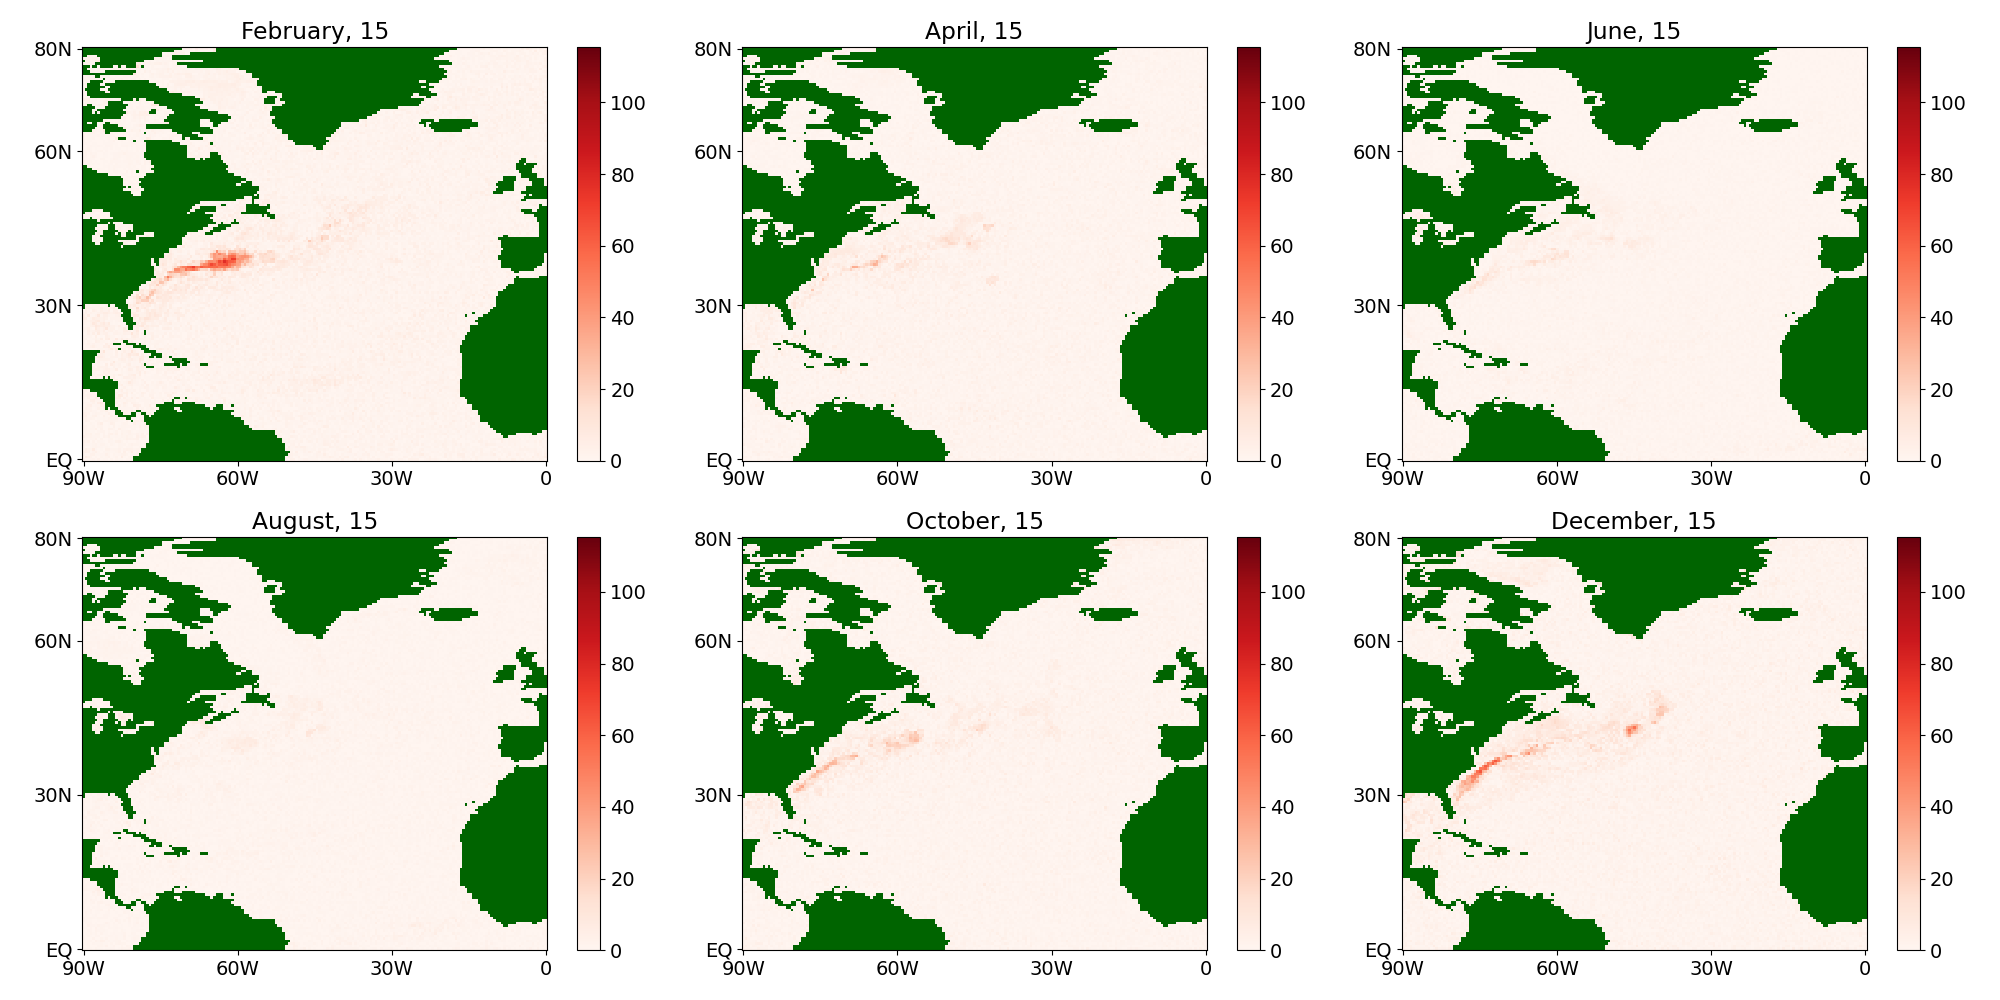
\includegraphics[width=\textwidth]{difference_a_compare_latent}
	\caption{Абсолютная разность оценок коэффициента дрейфа для скрытого потока в течение среднего года за период $1979-2022$ гг.} 
	\label{fig:latent_difference_a}
\end{figure}


\begin{figure}[!h]
	\centering
	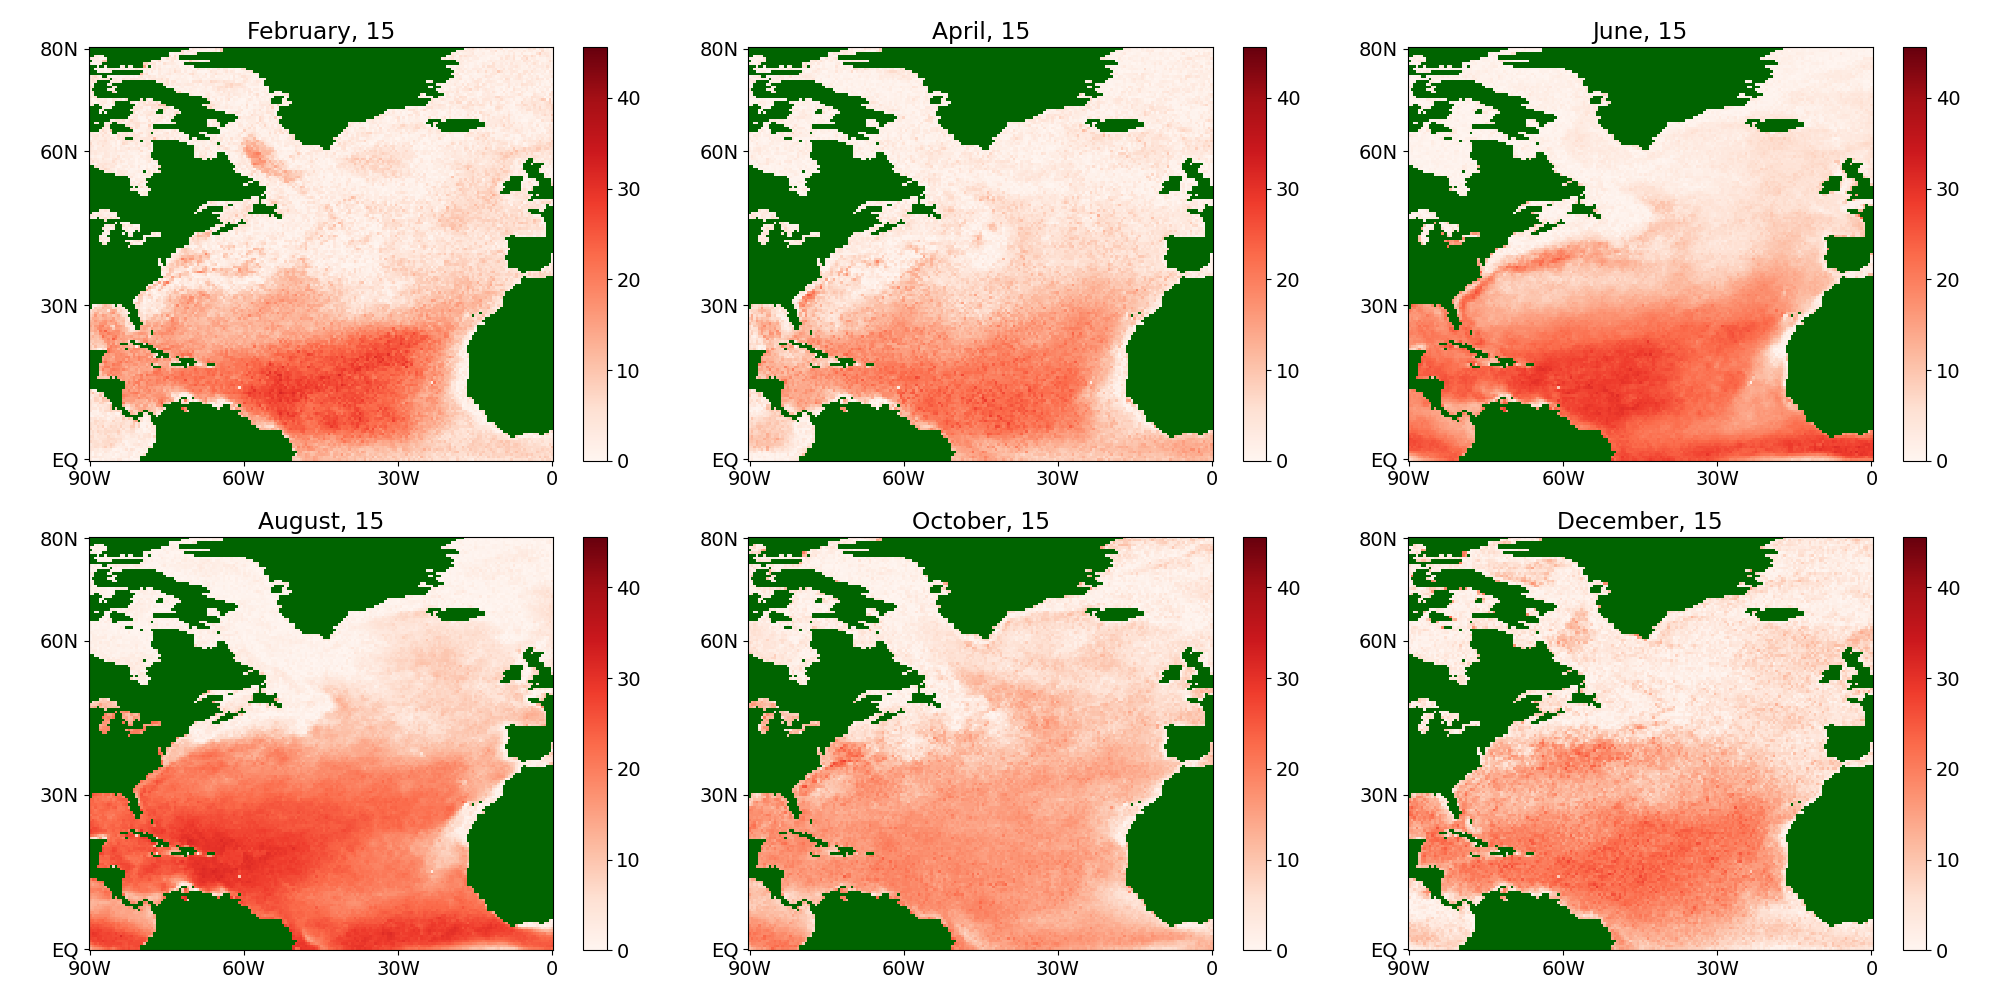
\includegraphics[width=\textwidth]{difference_b_compare_latent}
	\caption{Абсолютная разность оценок коэффициента диффузии для скрытого потока в течение среднего года за период $1979-2022$ гг.} 
	\label{fig:latent_difference_b}
\end{figure}

Для наглядного сравнения результатов, полученных обоими методами сразу для всей Северной Атлантики, значения абсолютных различий оценок в каждой точке полуградусной сетки представлены на рисунках \ref{fig:sensible_difference_a}-\ref{fig:latent_difference_b}. Снова используется формат среднего года.
Что касается коэффициентов дрейфа для потоков обоих типов, то вдоль Гольфстрима наблюдаются некоторые существенные различия в результатах применения методов (см. рисунки \ref{fig:sensible_difference_a} и \ref{fig:latent_difference_a}), в то время как для остальной части карты различия могут проявляться из-за погрешностей вычислений.

В то же время разница между полученными значениями коэффициента диффузии видна гораздо отчетливее (см. рисунки \ref{fig:sensible_difference_b} и \ref{fig:latent_difference_b}), особенно для зимы и весны среднего года в более северных широтах, а также в районе Гольфстрима. Этот факт может быть объяснен с геофизической точки зрения следующим образом. В северных широтах существует больше случайных факторов, определяющих взаимодействие океана и атмосферы, из–за большего разброса температур и более сильных ветров, которые в значительной степени определяют возникающие потоки тепла. Это один из наиболее важных аргументов в пользу более точной полупараметрической процедуры оценки (см. раздел \ref{sec:Semiparametric}).

В данном разделе были представлены результаты проведенных исследований по применению полупараметрического метода для восстановления коэффициентов случайного дрейфа $a(t,X)$ и диффузии $b(t,X)$ в СДУ Ито и сравнения этого метода с непараметрическим методом с использованием как синтетически сгенерированных данных, так и данных реанализа явного и скрытого потоков тепла в Северной Атлантике за период с $1979$ по $2022$ год из базы данных ERA5.

К преимуществам непараметрических процедур относится возможность теоретического доказательства свойств оценок, например, их согласованности, в том числе для многомерного случая. Однако этот метод требует нескольких дополнительных допущений. Процедура полупараметрической реконструкции свободна от них. Необходимо только наличие решения стохастического дифференциального уравнения. Однако этот метод ориентирован на выборки ограниченного объема (окна), что накладывает ограничения на возможность доказательства асимптотических статистических свойств. Однако эмпирическое сравнение обоих методов, приведенное ранее, показывает сходство их результатов, что указывает на возможность использования этих методов для прикладного математического моделирования.

\section{Разложение коэффициента диффузии на собственные вектора}
\label{sec:Karhunen}

В данном разделе описана методика применения разложения Карунена-Лоэва для полученных оценок коэффициента диффузии. Поскольку коэффициент диффузии имеет физическую интерпретацию суммарной энергии, заключенной в процессе, то его разложение на собственные вектора позволяет пролить свет на отдельные компоненты, из которых складывается эта энергия и выделить географические области наибольшей энергетической активности океана, что представляет большой интерес с точки зрения геофизики.

Модель~\eqref{eq:Ito} в дискретном виде может быть представлена в виде
\begin{equation}
	\label{eq:discrete_Ito}
	X(t+\Delta t) = a(t,X) \Delta t + b(t,X) (W (t+\Delta t)-W(t))	
\end{equation}
Здесь $X(t)$ и $a(t,X)$ - случайные векторы длиной $N$, $b(t,X)$ - матрица размера $N\times N$, а $W(t)$ -- Винеровский процесс, вектор длины $N$ с независимыми компонентами, который не зависит от процесса $X(t)$. Матрица $b(t,X)$ квадратная, невырожденная, положительно определенная и, следовательно, имеет полный набор собственных векторов $e_1,...,e_N$ и собственных значений $\lambda_1,...,\lambda_N$. Используя стандартный алгебраический метод декомпозиции по базису, из ~\eqref{eq:discrete_Ito} можно получить
\begin{equation}
	\label{eq:decomposition}
	X(t+\Delta t) = X(t) + a(t,X) \Delta t + \sum_{i=1}^N \lambda_i e_i \eta_i
\end{equation}
где $\eta_i= (e_i,W(t+\Delta t)-W(t))$ -- случайная величина, представляющая собой скалярное произведение векторов $e_i$ и $W(t+\Delta t)-W(t)$. Это гауссова случайная величина с нулевым средним значением и дисперсией, равной $\Delta t$, поскольку сумма составляющих вектора $e_i$ определяется однозначно из-за их ортонормированности. Вектор $W (t + \Delta t)-W (t)$ является гауссовым с независимыми компонентами и ковариационной матрицей с ненулевыми диагональными элементами, равными $\Delta t$. Чтобы проанализировать поведение приращений процесса $X(t+\Delta t) - X(t)$, необходимо изучить поведение коэффициента $a(t,X)$ и поведение собственных векторов $e_1,...,e_N$ и собственных значений $\lambda_1,...,\lambda_N$.


Для проведения данного разложения вновь необходимо предварительно произвести дискретизацию (см. раздел~\ref{sec:Discretization}) данных. Шкала значений временных рядов за достаточно длительный период времени ($10$ лет) разбивается на сегменты, вероятности попадания в которые случайно выбранных значений были бы максимально близки друг к другу. 

Далее выполняется алгоритм декомпозиции, который заключается в следующем:
\begin{itemize}
	\item Рассматриваются два временных ряда $X,Y$ (не обязательно различных, может быть $X \equiv Y$). Их значения зависят от выбора координаты точки сетки (с использованием одномерной проекции) и от рассматриваемого момента времени: $X=X(p,t), Y=Y(p,t)$. 
	\item Весь диапазон значений каждого из рядов разделяется на $n_{bins}=100$ непересекающихся и равновероятных (построенных с использованием квантилей) интервалов. Для каждой последующей пары моментов времени $(t,t+dt)$, где $dt$ равняется одному дню, выполняются следующие шаги:
	\begin{itemize}
		\item Создается ковариационная матрица $B$ размера $n_{bins} \times n_{bins}$.
		
		\item Для каждого интервала с номером $i_1$ $(0 \leqslant i_1 \leqslant n_{bins}-1)$ по первой переменной $X$ и независимо для каждого интервала с номером $j_1$ $(0 \leqslant j_1 \leqslant n_{bins}-1)$ по второй переменной $Y$ выбираются точки первого временного ряда в момент времени $t$, которые попадают в интервал $i_1$, обозначим их через $points_{x1}$ и для второго временного ряда в момент времени $t$, попадающего в интервал с номером $j_1$ ($points_{y1}$).
		
		\item Для этих точек вычисляются два вектора:
		\begin{equation*}
			vec_1 = X_{points_{x1},t+dt} - mean(X_{points_{x1},t}),\quad
			vec_2 = Y_{points_{y1},t+dt} - mean(Y_{points_{y1},t}).
		\end{equation*}
		Значения $mean(X[points_{x1},t]$) рассчитываются на основе оценок коэффициента дрейфа $a$.
		
		\item Вычисляется сумма произведений всех возможных пар этих двух векторов и присваивается соответствующему элементу матрицы $B$:
		\begin{equation*}
			B_{i_1, j_1} = \sum v_1 \cdot v_2, \quad v_1 \in vec_1, v2 \in vec_2.
		\end{equation*}
		Здесь неявно используется закон полной вероятности. Формально он требует учета вероятности переходов, как вероятностей элементов разбиения. Однако, поскольку в этом методе используется наиболее равновероятное деление всех значений на интервалы, вероятности попадания в каждый из интервалов примерно одинаковы, и различиями между ними можно пренебречь. %При этом учитывается размерность задачи, то есть берется матрица между значениями разных (либо одних и тех же) переменных.
		
		\item В случае различных переменных в паре $(X,Y)$ вместо матрицы $B$ рассмотрим матрицу $B^*$, полученную из следующего соотношения: ${B^*}^2= B \cdot B^T$.
		
		\item Построенная матрица $B$ раскладывается на собственные значения и векторы, которые затем упорядочиваются в порядке убывания модулей собственных значений: $\lambda_1,\dots,\lambda_{n_{bins}}$; $v_1,\dots,v_{n_{bins}}$.
		
		\item В паре $(\lambda_i, v_i)$ $\lambda_i$ -- число (вообще говоря, комплексное), а $v_i$ -- одномерный вектор длиной $n_{bins}$ (вообще говоря, комплексный). Собственное значение $\lambda_i$ соответствует второй переменной (временной ряд $Y$), что приводит к следующему правилу построения: 
		
		\item Создается пустая матрица (соответствующая географической карте исследуемой области) $M$ размером $161 \times 181$ точек. Для каждого интервала с номером $j_1$ $(0 \leqslant j_1 \leqslant n_{bins}-1)$ в соответствии со второй переменной $Y$ выполняется поиск точек второй строки в момент времени $t+dt$, попадающих в интервал с номером $j_2$: $points_{y2}$. Действительная часть соответствующего элемента собственного вектора с номером $j_2$ затем присваивается всем точкам этого множества: $M[points_{y2}] = v_i[j_2]$.
	\end{itemize}
\end{itemize}




